
\documentclass[12pt]{article}
%\input{preamble}
\usepackage{multirow}
\usepackage{amsmath}
\usepackage{fancyhdr}
\usepackage[left=1in,top=1.0in,right=1in,headsep=0.25in,footskip=0.3in,bottom=0.7in]{geometry}
%\usepackage[left=1in,top=1.2in,right=1in,footskip=0.3in,bottom=0.7in,showframe]{geometry}
%\usepackage[left=1in,top=1in,right=1in,bottom=1in,nohead]{geometry}
\usepackage{graphicx}
\renewcommand{\arraystretch}{1} % spacing between table rows
\usepackage[]{caption}
\setlength{\abovecaptionskip}{0pt}
\setlength{\belowcaptionskip}{-5pt}
\setlength{\intextsep}{10pt plus 2pt minus 2pt}
\usepackage[normalem]{ulem}
\newcounter{Labcounter}
\newcounter{Taskcounter}
\numberwithin{equation}{section}
\fancyhf{}


\usepackage{outlines}
\renewcommand{\theenumi}{\Roman{enumi}. }
\renewcommand{\labelenumi}{\theenumi}

\renewcommand{\theenumii}{\Alph{enumii}. }
\renewcommand{\labelenumii}{\theenumii}

\renewcommand{\theenumiii}{\roman{enumiii}. }
\renewcommand{\labelenumiii}{\theenumiii}

\renewcommand{\theenumiv}{\alph{enumiv}) }
\renewcommand{\labelenumiv}{\theenumiv}


%\usepackage{enumitem}

%\setenumerate[1]{label=\Roman*.}
%\setenumerate[2]{label=\Alph*.}
%\setenumerate[3]{label=\roman*.}
%\setenumerate[4]{label=\alph*.}



\usepackage[numbered,framed]{matlab-prettifier}

\lstMakeShortInline[style=Matlab-editor]"

\pagestyle{fancy}
\fancypagestyle{plain}{ %
% \fancyhf{} % remove everything
\renewcommand{\headrulewidth}{0pt} % remove lines as well
%\renewcommand{\footrulewidth}{0pt}
%\cfoot{Page \thepage~of \pageref{LastPage}}}
\cfoot{\thepage}
}

\newcommand{\blue}[1]{\textcolor{blue}{#1}} %for displaying red texts
\newcommand{\red}[1]{\textcolor{red}{[#1]}} %for displaying red texts

%\newcommand{\rood}[1]{} %for displaying red texts


\lhead{\textit{Nanocones...}}
%\chead{\Large \textbf{Paul W.~Leu } \vspace{0.3em}}
%\chead{\Large \textbf{NSF Biographical Sketch: Paul W.~Leu} \vspace{0.3em}}
\rhead{\textit{Leu}}


\newcommand{\vectornorm}[1]{\left|\left|#1\right|\right|}
%\usepackage[top=2.5cm, bottom=2.5cm, left=2.5cm, right=2.5cm]{geometry}
\usepackage[normalem]{ulem}
\newenvironment{packed_enum}{
\begin{enumerate}
  \setlength{\topsep}{0pt}
  \setlength{\partopsep}{0pt}
  \setlength{\itemsep}{1pt}
  \setlength{\parskip}{0pt}
  \setlength{\parsep}{0pt}
}{\end{enumerate}}

%\usepackage[small]{caption}
\usepackage[draft]{pdfcomment}
\usepackage{wrapfig}
\usepackage{hyperref}
\usepackage{paralist}
\usepackage{amsmath}
\usepackage{amssymb}
\usepackage{amsfonts}
\usepackage{textcomp}
\usepackage{subfig}
\usepackage{framed}
\usepackage{setspace}
\usepackage{here}
\usepackage[numbers, square, comma, sort&compress]{natbib}

\usepackage{mathtools}

\DeclareMathOperator{\lcm}{lcm}
\DeclarePairedDelimiter\floor{\lfloor}{\rfloor}

\usepackage[compact]{titlesec}
\titlespacing{\section}{0pt}{0ex}{0pt}
\titlespacing{\subsection}{0pt}{0pt}{0pt}
\usepackage{xcolor}

\usepackage[]{caption}
\setlength{\abovecaptionskip}{0pt}
\setlength{\belowcaptionskip}{-5pt}
\setlength{\intextsep}{10pt plus 2pt minus 2pt}

\defineavatar{Paul}{author=Paul,color=blue}
\defineavatar{Ziyu}{author=Ziyu,color=green}


\usepackage{float}
\floatstyle{plaintop}
\newfloat{program}{thp}{lop}
\floatname{program}{Table}

\newfloat{wrapprogram}{thp}{lop}
\floatname{wrapprogram}{Table}

%\setlength{\intextsep}{10pt plus 2pt minus 2pt}
% bold face: highlight keywords, or big ideas
% italics: inconspicuous stressing of key points
% underline: hypothesis; avoid

\usepackage{bm}

\date{\today }

\author{
Paul W. Leu\\
University of Pittsburgh\\
Pittsburgh, PA}


%\def\myTitle{CAREER: Transforming Solar Energy Harvesting through Nanophotonic Light Trapping}
%\def\myTitle{CAREER: Characterizing Enhanced Absorption and Carrier Collection Mechanisms in Silicon and Zinc Oxide Nanocone-based Solar Cells}
%Upper bound
%   100 hours/year
%    40 hours
%    
%\title{Ultimate Limits of Silicon Nanostructures for Photon Management\\
%\title{Determining Silicon/Metal Nanostructures that Approach the Wave-Optics Light Trapping Limit by Data Mining of Electrodynamic Simulations}
%\title{CAREER: Characterizing Enhanced Absorption and Carrier Collection Mechanisms in Silicon and Zinc Oxide Nanocone-based Solar Cells}
%\title{Predicting Wave-Optics Light Trapping in Silicon and Metal Nanostructure by Data Mining of Electrodynamic Simulations}
%Keywords: ultra thin, light trapping, wave-optics light trapping, coherent light trapping, optimization framework, data mining}

%\title{Modeling and Manufacturing of Three Dimensional Silicon Nanostructures for Photon Management}

\numberwithin{equation}{section}
\begin{document}
\tableofcontents

\begin{figure}[H]
\centering
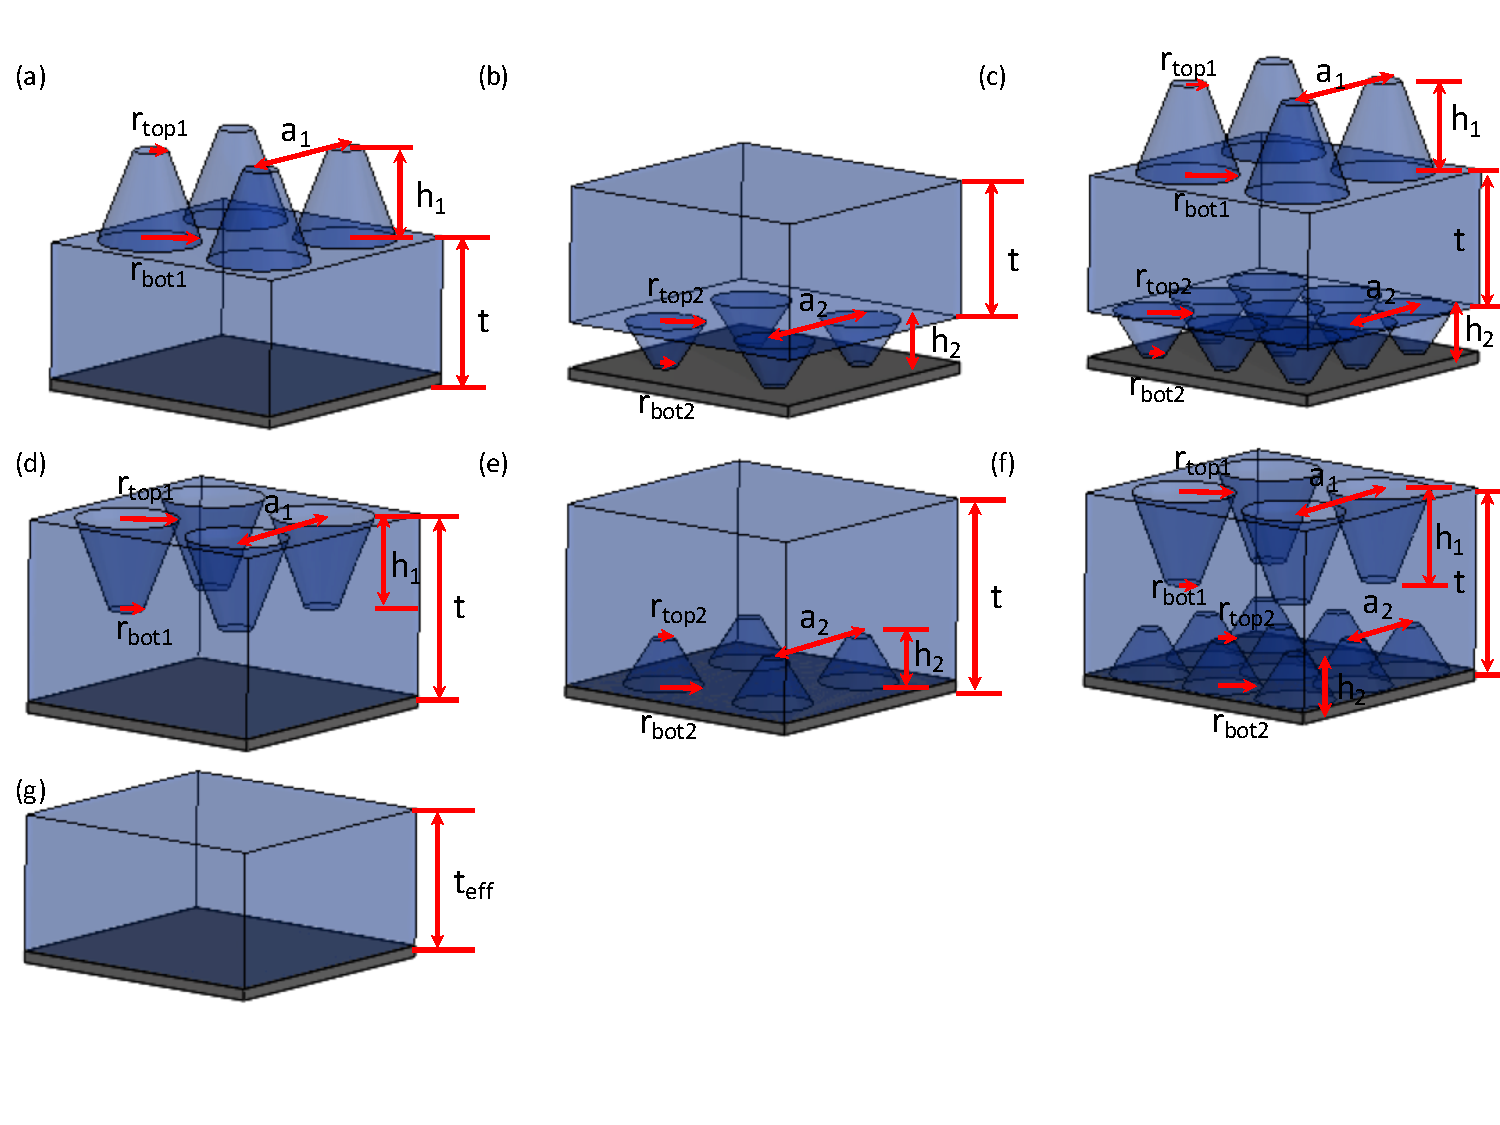
\includegraphics[scale=0.4]{../Figures/Schematic}
\caption{(a). Cone on the top (b). Cone on the bottom (c). Cone on  both top and bottom (d). Cone hole on the top (e). Cone hole on the bottom (f). Cone hole on both top and bottom}
\label{fig:Schematic}
\vspace{0pt}
\end{figure}
 
\section{Optimized Structures}
Figure~\ref{fig:Schematic} shows all the structures that will be optimized. \\ 
 \subsection{Cone on the top}
% \subsubsection{Five variables implementation}
%Figure~\ref{fig:Schematic} (a) shows nanocone structures on the top of a thin film.  
%The variables are $r_{top1}$, $r_{bot1}$, $a_1$,  $h_1$ and $t$.
%Let $\mathbf{x} = \left ( r_{top1}, r_{bot1}, a_1, h_1, t  \right )^T $.
%$a_{max}$ and $t_{eff}$ are set by the user.  To start with, we set $a_{max} = 4000$ nm, and $a_{min} = 100$ nm.  If we set $a_{min} = 0$, we should recover previous results.
%The bound constraints on the range of variables are
%\begin{align*}
%a_{min}/2 & \leq r_{top1} \leq a_{max}/2 \\
%a_{min}/2 & \leq r_{bot1} \leq a_{max}/2 \\
%a_{min} & \leq a_{1} \leq a_{max} \\
%0 & \leq h_{1} \leq   \frac{4 t_{eff}}{\pi} \frac{a_{max}^2}{a_{min}^2}  \\   % \infty \\
%0 & \leq t \leq t_{eff}
%\end{align*}
%We can express the bound constrains in matrix form as
%\begin{equation}
%\left(
%\begin{matrix}
%a_{min}/2\\ 
%a_{min}/2\\
%a_{min}\\ 
%0 \\    % \infty \\
%0 
%\end{matrix} \right )
%\leq \mathbf{x}
% \leq 
% \left(
%\begin{matrix}
%a_{max}/2 \\ a_{max}/2 \\ a_{max} \\  \frac{4 t_{eff}}{\pi} \frac{a_{max}^2}{a_{min}^2}  \\ t_{eff}
%\end{matrix} \right )
%\end{equation}
%The linear inequality constraints are 
%\begin{align*}   
%2r_{top1} \leq a_1 \\
%2r_{bot1} \leq a_1 
%\end{align*}
%The linear inequality constraints are of the form $\mathbf{A} \mathbf{x} \leq \mathbf{b}$.
%\begin{equation}
%\left(
%\begin{matrix}
%2 & 0 & -1 & 0 &  0 \\
%0 & 2 & -1 & 0 & 0 
%\end{matrix}
%\right ) \mathbf{x}  \leq \left ( \begin{matrix} 0\\ 0 \end{matrix} \right ) 
%\end{equation}
%
%The volume is unchanged during optimization, which results in a nonlinear constraint.
%\begin{align}
% a_{1}^2t_{eff} &= a_{1}^2t + \frac{1}{3}\pi h_1(r_{top1}^2+r_{bot1}^2+r_{top1}r_{bot1}) \nonumber \\
% t &= t_{eff} - \frac{1}{3 a_{1}^2}\pi h_1(r_{top1}^2+r_{bot1}^2+r_{top1}r_{bot1}) \nonumber \\
% h_1 &= \frac{3 a_1^2 (t_{eff} - t)}{\pi (r_{top1}^2+r_{bot1}^2+r_{top1}r_{bot1})}
% \end{align}
%The maximum $h_1$ occurs when $t = 0$, $a_1 = a_{max}$, and $r_{top1} = r_{bot1} = a_{min}/2$. The input $h_1$ is constrained by  the following condition and $h_1$ is always positive.
%\begin{equation*}
%h_{1} \leq \frac{4 t_{eff}}{\pi} \frac{a_{max}^2}{a_{min}^2}.
%\end{equation*}

%\subsubsection{Five Variable Matlab Implementation}
%
%Variables will be named "rTop1, rBot1, a1, h1," and "t."
%The filename of the simulation will be "[material.Type, 'NCToprTop1_', num2str(rTop1), 'rBot1_', num2str(rBot1), 'a1', num2str(a1), 'h1', num2str(h1), 't', num2str(t)]".
%
%
%\pdfcomment[avatar=Paul]{Please code Rectangle and Cone objects.}
%"classdef" \lstinputlisting[style=Matlab-editor]{@NCTop/NCTop.m}

\subsubsection{Four Variables Implementation}
The bound constraint conditions are the same as before without the constraint for  $h_1$.  Let $\mathbf{x} = \left ( r_{top1}, r_{bot1}, a_1, t  \right )^T $.
\subsubsection{Effective Thickness Constraint}
$a_{max}$ and $t_{eff}$ are set by the user.  To start with, we set $a_{max} = 4000$ nm, and $a_{min} = 100$ nm.  If we set $a_{min} = 0$, we should recover previous results.
The bound constraint conditions are the same as before without the constraint for  $h_1$.  Let $\mathbf{x} = \left ( r_{top1}, r_{bot1}, a_1, t  \right )^T $.


\begin{equation}
\left(
\begin{matrix}
a_{min}/2\\ 
a_{min}/2\\
a_{min}\\ 
0 
\end{matrix} \right )
\leq \mathbf{x}
 \leq 
 \left(
\begin{matrix}
a_{max}/2 \\ a_{max}/2 \\ a_{max}  \\ t_{eff}
\end{matrix} \right )
\end{equation}
The linear inequality constraints are 
\begin{align*}   
2r_{top1} \leq a_1 \\
2r_{bot1} \leq a_1 
\end{align*}
The linear inequality constraints are of the form $\mathbf{A} \mathbf{x} \leq \mathbf{b}$.
\begin{equation}
\left(
\begin{matrix}
2 & 0 & -1  &  0 \\
0 & 2 & -1 & 0 
\end{matrix}
\right ) \mathbf{x}  \leq \left ( \begin{matrix} 0\\ 0 \end{matrix} \right ) 
\end{equation}
The volume is unchanged during optimization, which results in the following derivation for the cone height $h_1$.  
\begin{align}
 a_{1}^2t_{eff} &= a_{1}^2t + \frac{1}{3}\pi h_1(r_{top1}^2+r_{bot1}^2+r_{top1}r_{bot1}) \nonumber \\
 t &= t_{eff} - \frac{1}{3 a_{1}^2}\pi h_1(r_{top1}^2+r_{bot1}^2+r_{top1}r_{bot1}) \nonumber \\
h_1 &= \frac{3 a_1^2 (t_{eff} - t)}{\pi (r_{top1}^2+r_{bot1}^2+r_{top1}r_{bot1})}
 \end{align}
 \begin{equation}
\boxed{h_1 = \frac{3 a_1^2 (t_{eff} - t)}{\pi (r_{top1}^2+r_{bot1}^2+r_{top1}r_{bot1})} }
 \end{equation}
 The minimum $h_1$ occurs when $t = t_{eff}$.  
The maximum $h_1$ occurs when $t = 0$, $a_1 = a_{max}$, and $r_{top1} = r_{bot1} = a_{min}/2$. The input $h_1$ is constrained by  the following condition and $h_1$ is always positive.
\begin{equation*}
0 \leq h_{1} \leq \frac{4 t_{eff}}{\pi} \frac{a_{max}^2}{a_{min}^2}.
\end{equation*}
%When it comes to the parameter $h_1$ which is eliminated in this case,  will be calculated from the other four variables.  
%\begin{equation}
% h_1 = \frac{3 a_1^2 (t_{eff} - t)}{\pi (r_{top1}^2+r_{bot1}^2+r_{top1}r_{bot1})}
%\end{equation}
%With the other constraints in place, the constraints on $h_1$ will automatically be satisfied. In this way, the optimization could be simplified.  \\

\subsubsection{Total Thickness Constraint Implementation}
Here we provide another method of setting constraints for optimization.
Instead of constraining the optimization based on effective thickness, $t_{eff}$, we constrain the total thickness $t_{tot}$ where $h_1 + t = t_{tot}$.  
%$h_1$, also there are four input variables, $r_{top1}$, $r_{bot1}$, $a_1$ and $t$.
Let $\mathbf{x} = \left ( r_{top1}, r_{bot1}, a_1, t  \right )^T $.
$a_{max}$ and $t_{total}$ are set by the user.  To start with, we set $a_{max} = 4000$ nm, $a_{min} = 100$ nm, $t_{total} = 1000 nm$.  If we set $a_{min} = 0$, we should recover previous results.
The bound constraints on the range of variables are
\begin{align*}
a_{min}/2 & \leq r_{top1} \leq a_{max}/2 \\
a_{min}/2 & \leq r_{bot1} \leq a_{max}/2 \\
a_{min} & \leq a_{1} \leq a_{max} \\
0 & \leq t \leq t_{total}
\end{align*}
We can express the bound constrains in matrix form as
\begin{equation}
\left(
\begin{matrix}
a_{min}/2\\ 
a_{min}/2\\
a_{min}\\ 
0 
\end{matrix} \right )
\leq \mathbf{x}
 \leq 
 \left(
\begin{matrix}
a_{max}/2 \\ a_{max}/2 \\ a_{max} \\  t_{total}
\end{matrix} \right )
\end{equation}
The linear inequality constraints are 
\begin{align*}   
2r_{top1} \leq a_1 \\
2r_{bot1} \leq a_1 
\end{align*}
The linear inequality constraints are of the form $\mathbf{A} \mathbf{x} \leq \mathbf{b}$.
\begin{equation}
\left(
\begin{matrix}
2 & 0 & -1 & 0  \\
0 & 2 & -1 & 0 
\end{matrix}
\right ) \mathbf{x}  \leq \left ( \begin{matrix} 0\\ 0 \end{matrix} \right ) 
\end{equation}
The summation of cone height $h_1$ and thin film thickness $t$ should be equals to pre-setting $t_{total}$, which results in a different constraint from previous section.
\begin{align}
 h_{1} + t &= t_{total} \nonumber \\
 h_{1} &= t_{total}-t 
 \end{align}
 \begin{equation}
 \boxed{h_1 = t_{total} - t}
 \end{equation}
From the equation above, we know the $h_1$ will be smaller than $t_{total}$ by itself and it is always positive. 
\begin{equation}
0 \leq h \leq t_{total}
\end{equation}
No additional constraints must be implemented for $h_1$.  \\

\subsection{Cone on the bottom}
%\subsubsection{Five Variables Implementation}
% 
%Figure~\ref{fig:Schematic} (b) shows nanocone structures on the bottom of the thin film.  
%The input five variables are $r_{top2}$, $r_{bot2}$, $a_2$, $h_2$ and $t$.  
%Let $\mathbf{x} = \left ( r_{top2}, r_{bot2}, a_2, h_2, t  \right )^T$.
%$a_{max}$ and $t_{eff}$ are set by the user.  To start with, we set $a_{max} = 4000$ nm, and $a_{min} = 100$ nm.  If we set $a_{min} = 0$, we should recover previous results.
%The bound constraints on the range of variables are
%\begin{align*}
%a_{min}/2 & \leq r_{top2} \leq a_{max}/2 \\
%a_{min}/2 & \leq r_{bot2} \leq a_{max}/2 \\
%a_{min} & \leq a_{2} \leq a_{max} \\
%0 & \leq h_2 \leq \frac{4 t_{eff}}{\pi} \frac{a_{max}^2}{a_{min}^2}  \\
%0 & \leq t \leq t_{eff}
%\end{align*}
%We can express the bound constrains in matrix form as
%\begin{equation}
%\left(
%\begin{matrix}
%a_{min}/2\\ 
%a_{min}/2\\
%a_{min}\\ 
%0 \\    % \infty \\
%0 
%\end{matrix} \right )
%\leq \mathbf{x}
% \leq 
% \left(
%\begin{matrix}
%a_{max}/2 \\ a_{max}/2 \\ a_{max} \\  \frac{4 t_{eff}}{\pi} \frac{a_{max}^2}{a_{min}^2}  \\ t_{eff}
%\end{matrix} \right )
%\end{equation}
%The linear inequality constraints are 
%\begin{align*} 
%2r_{top2} \leq a_2 \\
%2r_{bot2} \leq a_2 
%\end{align*}
%Linear inequality constraints are of the form $\mathbf{A} \mathbf{x} \leq \mathbf{b}$.
%\begin{equation}
%\left(
%\begin{matrix}
%2 & 0 & -1 & 0 & 0 \\
%0 & 2 & -1 & 0 & 0 \\
%\end{matrix}
%\right ) \mathbf{x}  \leq \left ( \begin{matrix} 0\\ 0 \end{matrix} \right ) 
%\end{equation}
%The volume is unchanged during optimization, which results in a nonlinear constraint
%\begin{align}
% a_{2}^2 t_{eff} &= a_{2}^2 t + \frac{1}{3}\pi h_2(r_{top2}^2+r_{bot2}^2+r_{top2}r_{bot2})\nonumber \\
% t &= t_{eff} - \frac{1}{3 a_{2}^2}\pi h_2(r_{top2}^2+r_{bot2}^2+r_{top2}r_{bot2})\nonumber \\
% h_2 &= \frac{3 a_2^2 (t_{eff} - t)}{\pi (r_{top2}^2+r_{bot2}^2+r_{top2}r_{bot2})}
%\end{align}
%The maximum $h_2$ occurs when $t = 0$, $a_2 = a_{max}$, and $r_{top2} = r_{bot2} = a_{min}/2$. The input $h_2$ is constrained by  the following condition and we know $h_2$ is always positive from the equation.
%\begin{equation*}
%h_{2} \leq \frac{4 t_{eff}}{\pi} \frac{a_{max}^2}{a_{min}^2}
%\end{equation*}

\subsubsection{Effective Thickness Constraint Implementation}
The constraints are exactly the same as in the above case, except all the structures are on the bottom as opposed to the top.
The bound constraint conditions are similar as before without the input variable $h_2$.  
Let $\mathbf{x} = \left ( r_{top2}, r_{bot2}, a_2, t  \right )^T $.

\begin{equation}
\left(
\begin{matrix}
a_{min}/2\\ 
a_{min}/2\\
a_{min}\\ 
0 
\end{matrix} \right )
\leq \mathbf{x}
 \leq 
 \left(
\begin{matrix}
a_{max}/2 \\ a_{max}/2 \\ a_{max}  \\ t_{eff}
\end{matrix} \right )
\end{equation}
The linear inequality constraints are 
\begin{align*}   
2r_{top2} \leq a_2 \\
2r_{bot2} \leq a_2 
\end{align*}
The linear inequality constraints are of the form $\mathbf{A} \mathbf{x} \leq \mathbf{b}$.
\begin{equation}
\left(
\begin{matrix}
2 & 0 & -1  &  0 \\
0 & 2 & -1 & 0 
\end{matrix}
\right ) \mathbf{x}  \leq \left ( \begin{matrix} 0\\ 0 \end{matrix} \right ) 
\end{equation}
%When it comes to the parameter $h_1$ which is eliminated in this case,  will be calculated from the other four variables.  
$h_2$ may be calculated from the other four variables.  
\begin{equation}
 h_2 = \frac{3 a_2^2 (t_{eff} - t)}{\pi (r_{top2}^2+r_{bot2}^2+r_{top2}r_{bot2})}
\end{equation}
With the other constraints in place, the constraints on $h_2$ will automatically be satisfied. In this way, the optimization could be simplified.  \\

\subsubsection{Total Thickness Constraint Implementation}
For this case, it is similar to the previous conetop structure, also there are four input variables, $r_{top2}$, $r_{bot2}$, $a_2$ and $t$.
Let $\mathbf{x} = \left ( r_{top2}, r_{bot2}, a_2, t  \right )^T $.
$a_{max}$ and $t_{total}$ are set by the user.  To start with, we set $a_{max} = 4000$ nm, $a_{min} = 100$ nm, $t_{total} = 1000$ nm.  If we set $a_{min} = 0$, we should recover previous results.
The bound constraints on the range of variables are
\begin{align*}
a_{min}/2 & \leq r_{top2} \leq a_{max}/2 \\
a_{min}/2 & \leq r_{bot2} \leq a_{max}/2 \\
a_{min} & \leq a_{2} \leq a_{max} \\
0 & \leq t \leq t_{total}
\end{align*}
We can express the bound constrains in matrix form as
\begin{equation}
\left(
\begin{matrix}
a_{min}/2\\ 
a_{min}/2\\
a_{min}\\ 
0 
\end{matrix} \right )
\leq \mathbf{x}
 \leq 
 \left(
\begin{matrix}
a_{max}/2 \\ a_{max}/2 \\ a_{max} \\  t_{total}
\end{matrix} \right )
\end{equation}
The linear inequality constraints are 
\begin{align*}   
2r_{top2} \leq a_1 \\
2r_{bot2} \leq a_1 
\end{align*}
The linear inequality constraints are of the form $\mathbf{A} \mathbf{x} \leq \mathbf{b}$.
\begin{equation}
\left(
\begin{matrix}
2 & 0 & -1 & 0  \\
0 & 2 & -1 & 0 
\end{matrix}
\right ) \mathbf{x}  \leq \left ( \begin{matrix} 0\\ 0 \end{matrix} \right ) 
\end{equation}
The summation of cone height $h_1$ and thin film thickness $t$ should be equals to pre-setting $t_{total}$, which results in a different constraint from previous section.
\begin{align}
 h_{2} + t &= t_{total} \nonumber \\
 h_{2} = t_{total}-t 
 \end{align}
From the equation above, we know the $h_2$ will be smaller than $t_{total}$ by itself and it is always positive. \\

\subsection{Cone on both top and bottom}
Figure~\ref{fig:Schematic} (c) shows nanocone structures on both top and bottom of the thin film. For this complicated structure, we first have the case where we assume the pitches on the top and bottom are the same before relaxing this assumption.  
%make two assumptions, symmetric and asymmetric cone on both sides. 
\subsubsection{Cone Arrays  with Same Pitch on Both Top and Bottom}
In this section, we make assumption that the periodicity of the cones on top $a_1$ and the periodicity of the cones on the bottom are equal to one another, or $a_1 = a_2 = a$.   
\begin{outline}[enumerate]
%\1 \textbf{Eight Variables Implementation} \\
%Let's consider the simple situation. To optimize the cone structures, we input the eight variables, $r_{top1}$, $r_{top2}$, $r_{bot1}$, $r_{bot2}$, $a$, $h_1$, $h_2$, and $t$. $a_{min}$, $a_{max}$ and $t_{eff}$ are set by the user. Let $\mathbf{x} = \left ( r_{top1}, r_{bot1}, r_{top2}, r_{bot2}, a, h_1, h_2, t  \right )^T $. To start with, we set $a_{max} = 4000$ nm, $a_{min} = 100$ nm.  and $t_{eff} = 1000$ nm. If we set $a_{min} = 0$, we should recover previous results.
%The bound constraints on the range of variables are
%\begin{align*}
%a_{min}/2 & \leq r_{top1} \leq a_{max}/2 \\
%a_{min}/2 & \leq r_{bot1} \leq a_{max}/2 \\
%a_{min}/2 & \leq r_{top2} \leq a_{max}/2 \\
%a_{min}/2 & \leq r_{bot2} \leq a_{max}/2 \\
%%0 & \leq a \leq a_{max} \\
%a_{min} & \leq a\leq a_{max} \\
%0 & \leq h_1 \leq \frac{4 t_{eff}}{\pi}  \\
%0 & \leq h_2 \leq \frac{4 t_{eff}}{\pi}  \\
%0 & \leq t \leq t_{eff}
%\end{align*}
%We can express the bound constrains in matrix form as follow
%\begin{equation}
%\left(
%\begin{matrix}
%a_{min}/2\\ 
%a_{min}/2\\ 
%a_{min}/2\\ 
%a_{min}/2\\
%a_{min}\\ 
%0 \\
%0 \\
%0 
%\end{matrix} \right )
%\leq \mathbf{x}
% \leq 
% \left(
%\begin{matrix}
%a_{max}/2 \\ a_{max}/2 \\ a_{max}/2 \\ a_{max}/2 \\ a_{max} \\ \frac{4 t_{eff}}{\pi}  \\\frac{4 t_{eff}}{\pi} \\t_{eff}
%\end{matrix} \right )
%\end{equation}
%The linear inequality constraints are 
%\begin{align*} 
%2r_{top1} \leq a \\
%2r_{bot1} \leq a\\
%2r_{top2} \leq a\\
%2r_{bot2} \leq a 
%\end{align*}
%Linear inequality constraints are of the form $\mathbf{A} \mathbf{x} \leq \mathbf{b}$.
%\setcounter{MaxMatrixCols}{20}
%\begin{equation}
%\left(
%\begin{matrix}
%2 & 0 & 0 & 0 & -1 & 0 & 0 & 0 & 0  \\
%0 & 2 & 0 & 0 & -1 & 0 & 0 & 0 & 0 \\
%0 & 0 & 2 & 0 & -1 & 0 & 0 & 0 & 0 \\
%0 & 0 & 0 & 2 & -1& 0 & 0 & 0 & 0 
%\end{matrix}
%\right ) \mathbf{x}  \leq \left ( \begin{matrix} 0\\ 0\\ 0\\ 0 \end{matrix} \right ) 
%\end{equation}
%The volume must be unchanged during simulation:
%\begin{align}
%a^2 t_{eff} &= a^2 t + \frac{1}{3}\pi h_1(r_{top1}^2+r_{bot1}^2+r_{top1}r_{bot1})+\frac{1}{3}\pi h_2(r_{top2}^2+r_{bot2}^2+r_{top2}r_{bot2})\nonumber \\
%t &= t_{eff} - \frac{1}{3a^2}\pi h_1(r_{top1}^2+r_{bot2}^2+r_{top2}r_{bot2}) - \frac{1}{3a^2}\pi h_2(r_{top2}^2+r_{bot2}^2+r_{top2}r_{bot2})
% \end{align}  \\
%The maximum $t$ occurs when $h_{1}$ and $h_{2}$ are 0. $t=t_{eff}$. \\
%The maximum $h_1$ occurs when $h_{2}=0$, $t = 0$ and $r_{top1} = r_{bot1} = a_1/2$.  
%\begin{align*}
%0 &= t_{eff} - \frac{1}{4}\pi h_1 \\
%h_{1} &\leq \frac{4 t_{eff}}{\pi}  
%\end{align*}
%The maximum $h_2$ occurs when $h_{1}=0$, $t = 0$ and $r_{top2} = r_{bot2} = a_2/2$.  
%%\red{Shouldn't this be when $t = 0$?}
%\begin{equation*}
%h_{2} \leq \frac{4 t_{eff}}{\pi} 
%\end{equation*}
%The following must be implemented as a nonlinear constraint:
%\begin{equation}
%\boxed{t = t_{eff} - \frac{1}{3a^2}\pi h_1(r_{top1}^2+r_{bot2}^2+r_{top2}r_{bot2}) - \frac{1}{3a^2}\pi h_2(r_{top2}^2+r_{bot2}^2+r_{top2}r_{bot2})}
%\end{equation}


\1 \textbf{Seven Variables Implementation} \\
For this section, we are trying to reduce one more variable from the input variables, such as $t$.  
Thus the variables are $r_{top1}$, $r_{top2}$, $r_{bot1}$, $r_{bot2}$, $a$, $h_1$, and $h_2$. \\
Let $\mathbf{x} = \left ( r_{top1}, r_{bot1}, r_{top2}, r_{bot2}, a, h_1, h_2  \right )^T $. \\
$a_{min}$, $a_{max}$ and $t_{eff}$ are set by the user.   To start with, we set $a_{max} = 4000$ nm, $a_{min} = 100$ nm and $t_{eff} = 1000$nm.  If we set $a_{min} = 0$, we should recover previous results.
The bound constraints on the range of variables are

\begin{align*}
a_{min}/2 & \leq r_{top1} \leq a_{max}/2 \\
a_{min}/2 & \leq r_{bot1} \leq a_{max}/2 \\
a_{min}/2 & \leq r_{top2} \leq a_{max}/2 \\
a_{min}/2 & \leq r_{bot2} \leq a_{max}/2 \\
a_{min} & \leq a \leq a_{max} \\
0 & \leq h_1 \leq \frac{4 t_{eff}}{\pi}  \\
0 & \leq h_2 \leq \frac{4 t_{eff}}{\pi}
%0 & \leq t \leq t_{eff}
\end{align*}

We can express the bound constrains in matrix form as follow
\begin{equation}
\left(
\begin{matrix}
a_{min}/2\\ 
a_{min}/2\\ 
a_{min}/2\\ 
a_{min}/2\\
a_{min}\\ 
0 \\
0 
\end{matrix} \right )
\leq \mathbf{x}
 \leq 
 \left(
\begin{matrix}
a_{max}/2 \\ a_{max}/2 \\ a_{max}/2 \\ a_{max}/2 \\ a_{max} \\ \frac{4 t_{eff}}{\pi} \\ \frac{4 t_{eff}}{\pi}
\end{matrix} \right )
\end{equation}
The linear inequality constraints are 
\begin{align*} 
2r_{top1} \leq a \\
2r_{bot1} \leq a\\
2r_{top2} \leq a\\
2r_{bot2} \leq a 
\end{align*}
Linear inequality constraints are of the form $\mathbf{A} \mathbf{x} \leq \mathbf{b}$.
\setcounter{MaxMatrixCols}{20}
\begin{equation}
\left(
\begin{matrix}
2 & 0 & 0 & 0 & -1 & 0 & 0  \\
0 & 2 & 0 & 0 & -1 & 0 & 0 \\
0 & 0 & 2 & 0 & -1& 0 & 0 \\
0 & 0 & 0 & 2 & -1& 0 & 0
\end{matrix}
\right ) \mathbf{x}  \leq \left ( \begin{matrix} 0\\ 0\\ 0\\ 0 \end{matrix} \right ) 
\end{equation}
\begin{align}
a^2 t_{eff} &= a^2 t + \frac{1}{3}\pi h_1(r_{top1}^2+r_{bot1}^2+r_{top1}r_{bot1})+\frac{1}{3}\pi h_2(r_{top2}^2+r_{bot2}^2+r_{top2}r_{bot2})\nonumber \\
t &= t_{eff} - \frac{1}{3a^2}\pi h_1(r_{top1}^2+r_{bot2}^2+r_{top2}r_{bot2}) - \frac{1}{3a^2}\pi h_2(r_{top2}^2+r_{bot2}^2+r_{top2}r_{bot2})
 \end{align} 
\begin{equation}
\boxed{t = t_{eff} - \frac{1}{3a^2}\pi h_1(r_{top1}^2+r_{bot2}^2+r_{top2}r_{bot2}) - \frac{1}{3a^2}\pi h_2(r_{top2}^2+r_{bot2}^2+r_{top2}r_{bot2})}
\end{equation}
The maximum $t$ occurs when $h_{1}$ and $h_{2}$ are 0 or $t_{max}=t_{eff}$.  
The minimum $t$ occurs when $h_{1}$ or $h_{2}$ reaches the maximum, then the $t$ = 0.
%The other constraint on $t$ is satisfied based on constraints


%Then we find the maximum of $h_1$ and $h_2$, inserting them into equation, t is always positive. \\

\1 \textbf{Total Thickness Constraint Implementation} \\
For this section, we are trying to use another way to do with the constraints and reduce one more variable from the input variables, such as $t$.  
Thus the variables are $r_{top1}$, $r_{top2}$, $r_{bot1}$, $r_{bot2}$, $a$, $h_1$, and $h_2$. \\
Let $\mathbf{x} = \left ( r_{top1}, r_{bot1}, r_{top2}, r_{bot2}, a, h_1, h_2  \right )^T $. \\
%\red{Why not eliminate $t$ instead of $h_2$ like in previous example?} 
$a_{min}$, $a_{max}$ and $t_{total}$ are set by the user.   To start with, we set $a_{max} = 4000$ nm, $a_{min} = 100$ nm and $t_{total} = 1000$nm.  If we set $a_{min} = 0$, we should recover previous results.
The bound constraints on the range of variables are
\begin{align*}
a_{min}/2 & \leq r_{top1} \leq a_{max}/2 \\
a_{min}/2 & \leq r_{bot1} \leq a_{max}/2 \\
a_{min}/2 & \leq r_{top2} \leq a_{max}/2 \\
a_{min}/2 & \leq r_{bot2} \leq a_{max}/2 \\
a_{min} & \leq a \leq a_{max} \\
0 & \leq h_1 \leq t_{total} \\
0 & \leq h_2 \leq t_{total}
\end{align*}

We can express the bound constrains in matrix form as follow
\begin{equation}
\left(
\begin{matrix}
a_{min}/2\\ 
a_{min}/2\\ 
a_{min}/2\\ 
a_{min}/2\\
a_{min}\\ 
0 \\
0 
\end{matrix} \right )
\leq \mathbf{x}
 \leq 
 \left(
\begin{matrix}
a_{max}/2 \\ a_{max}/2 \\ a_{max}/2 \\ a_{max}/2 \\ a_{max} \\ t_{total} \\t_{total}
\end{matrix} \right )
\end{equation}
The linear inequality constraints are 
\begin{align*} 
2r_{top1} \leq a \\
2r_{bot1} \leq a \\
2r_{top2} \leq a \\
2r_{bot2} \leq a \\
h_1+h_2 \leq t_{total} 
\end{align*}
Linear inequality constraints are of the form $\mathbf{A} \mathbf{x} \leq \mathbf{b}$.
\setcounter{MaxMatrixCols}{20}
\begin{equation}
\left(
\begin{matrix}
2 & 0 & 0 & 0 & -1 & 0 & 0  \\
0 & 2 & 0 & 0 & -1 & 0 & 0 \\
0 & 0 & 2 & 0 & -1& 0 & 0 \\
0 & 0 & 0 & 2 & -1& 0 & 0 \\
0 & 0 & 0 & 0 & 0 & 1 & 1
\end{matrix}
\right ) \mathbf{x}  \leq \left ( \begin{matrix} 0\\ 0\\ 0\\ 0\\ t_{total} \end{matrix} \right ) 
\end{equation}
All the structure is optimized in a range of thickness $t_{total}$, the input variables $t$ and $h_1$ should be positve, thus $h_2$ is positive and automatically smaller than $t_{total}$. 
\begin{align}
h_1+h_2+t=t_{total} \nonumber \\
t=t_{total}-h_1-h_2
 \end{align} 
 
 \begin{equation}
\boxed{t=t_{total}-h_1-h_2}
 \end{equation}
 Using linear constraint, we have
\begin{equation}
0 \leq t \leq t_{total}
\end{equation}

%\red{If we use 8 variables, can just implement everything with linear constraint.  Think better to implement with $h_1 + h_2 + t = t_{total}$.  Think if you implement the way you have written, $t$ will be biased towards small values.}
 
 \1 \textbf{Total Thickness Constraint Implementation} \\
 \textbf{Eight Variables Implementation Optional} \\
It is an optional section for 8 input variables and with linear constraints.  The variables are $r_{top1}$, $r_{top2}$, $r_{bot1}$, $r_{bot2}$, $a$, $h_1$, $h_2$, and  $t$. \\
Let $\mathbf{x} = \left ( r_{top1}, r_{bot1}, r_{top2}, r_{bot2}, a, h_1, h_2, t \right )^T $. \\
%\red{Why not eliminate $t$ instead of $h_2$ like in previous example?} 
$a_{min}$, $a_{max}$ and $t_{total}$ are set by the user.   To start with, we set $a_{max} = 4000$ nm, $a_{min} = 100$ nm and $t_{total} = 1000$nm.  If we set $a_{min} = 0$, we should recover previous results.
The bound constraints on the range of variables are
\begin{align*}
a_{min}/2 & \leq r_{top1} \leq a_{max}/2 \\
a_{min}/2 & \leq r_{bot1} \leq a_{max}/2 \\
a_{min}/2 & \leq r_{top2} \leq a_{max}/2 \\
a_{min}/2 & \leq r_{bot2} \leq a_{max}/2 \\
a_{min} & \leq a \leq a_{max} \\
0 & \leq h_1 \leq t_{total} \\
0 & \leq h_2 \leq t_{total} \\
0 & \leq t \leq t_{total}
\end{align*}

We can express the bound constrains in matrix form as follow
\begin{equation}
\left(
\begin{matrix}
a_{min}/2\\ 
a_{min}/2\\ 
a_{min}/2\\ 
a_{min}/2\\
a_{min}\\ 
0 \\
0 \\
0 
\end{matrix} \right )
\leq \mathbf{x}
 \leq 
 \left(
\begin{matrix}
a_{max}/2 \\ a_{max}/2 \\ a_{max}/2 \\ a_{max}/2 \\ a_{max} \\ t_{total} \\t_{total}
\end{matrix} \right )
\end{equation}
The linear inequality constraints are 
\begin{align*} 
2r_{top1} \leq a \\
2r_{bot1} \leq a \\
2r_{top2} \leq a \\
2r_{bot2} \leq a \\
h_1+h_2+t \leq t_{total} 
\end{align*}
Linear inequality constraints are of the form $\mathbf{A} \mathbf{x} \leq \mathbf{b}$.
\setcounter{MaxMatrixCols}{20}
\begin{equation}
\left(
\begin{matrix}
2 & 0 & 0 & 0 & -1 & 0 & 0 &0  \\
0 & 2 & 0 & 0 & -1 & 0 & 0 &0\\
0 & 0 & 2 & 0 & -1& 0 & 0 &0\\
0 & 0 & 0 & 2 & -1& 0 & 0 &0\\
0 & 0 & 0 & 0 & 0 & 1 & 1 &1
\end{matrix}
\right ) \mathbf{x}  \leq \left ( \begin{matrix} 0\\ 0\\ 0\\ 0\\ t_{total} \end{matrix} \right ) 
\end{equation}
All the structure is optimized in a range of thickness $t_{total}$, the input variables $t$, $h_1$and $h_2$ should be positive. Since all of them are positive, then by the constraint showing below, they could not larger than $t_{total}$
\begin{align}
\boxed{h_1+h_2+t=t_{total} }
 \end{align} 
 
% \begin{equation}
%\boxed{t=t_{total}-h_1-h_2}
 %\end{equation}
 %Using linear constraint, we have
%\begin{equation}
%0 \leq t \leq t_{total}
%\end{equation}

%\red{If we use 8 variables, can just implement everything with linear constraint.  Think better to implement with $h_1 + h_2 + t = t_{total}$.  Think if you implement the way you have written, $t$ will be biased towards small values.} 
 
 
\end{outline}

\subsubsection{Cone Arrays with Different Pitches on Both Top and Bottom}
\begin{outline}[enumerate]
\1 \textbf{Eleven Variables Implementation} \\
Figure~\ref{fig:Schematic} (c) shows nanocone structures on both top and bottom of a thin film.  
The variables are $r_{top1}$, $r_{top2}$, $r_{bot1}$, $r_{bot2}$, $a_1$, $a_2$, $n_1$, $n_2$ , $h_1$, $h_2$, and $t$. \\
Let $\mathbf{x} = \left ( r_{top1}, r_{bot1}, r_{top2}, r_{bot2}, a_1, a_2, n_1, n_2, h_1, h_2, t  \right )^T $. \\
$a_{max}$, $n_{max}$ and $t_{eff}$ are set by the user.  $n_{1}$ and $n_{2}$ are integers. To start with, we set $a_{max} = 4000$ nm.
%, $n_{max} = 10$.
We can set $a_{min} = 100$ nm.  If we set $a_{min} = 0$, we should recover previous results.
$n_{max} = \floor{a_{max}/a_{min}}$, where $\floor{ }$ denotes the floor function.

The bound constraints on the range of variables are
\begin{align*}
a_{min}/2 & \leq r_{top1} \leq a_{max}/2 \\
a_{min}/2 & \leq r_{bot1} \leq a_{max}/2 \\
a_{min}/2 & \leq r_{top2} \leq a_{max}/2 \\
a_{min}/2 & \leq r_{bot2} \leq a_{max}/2 \\
%0 & \leq a \leq a_{max} \\
a_{min} & \leq a_{1} \leq a_{max} \\
a_{min} & \leq a_{2} \leq a_{max} \\
1 & \leq n_1 \leq  \floor{a_{max}/a_{min}} \\
1 & \leq n_2 \leq  \floor{a_{max}/a_{min}} \\
0 & \leq h_1 \leq \frac{4 t_{eff}}{\pi}  \\
0 & \leq h_2 \leq \frac{4 t_{eff}}{\pi}  \\
0 & \leq t \leq t_{eff}
\end{align*}

We can express the bound constrains in matrix form as follow
\begin{equation}
\left(
\begin{matrix}
a_{min}/2\\ 
a_{min}/2\\ 
a_{min}/2\\ 
a_{min}/2\\
a_{min}\\ 
a_{min}\\ 
1 \\    % \infty \\
1 \\
0 \\
0 \\
0 
\end{matrix} \right )
\leq \mathbf{x}
 \leq 
 \left(
\begin{matrix}
a_{max}/2 \\ a_{max}/2 \\ a_{max}/2 \\ a_{max}/2 \\ a_{max} \\ a_{max} \\  \floor{a_{max}/a_{min}} \\  \floor{a_{max}/a_{min}} \\ \frac{4 t_{eff}}{\pi}  \\\frac{4 t_{eff}}{\pi} \\t_{eff}
\end{matrix} \right )
\end{equation}
The linear inequality constraints are 
\begin{align*} 
2r_{top1} \leq a_1 \\
2r_{bot1} \leq a_1\\
2r_{top2} \leq a_2\\
2r_{bot2} \leq a_2 
\end{align*}
Linear inequality constraints are of the form $\mathbf{A} \mathbf{x} \leq \mathbf{b}$.
\setcounter{MaxMatrixCols}{20}
\begin{equation}
\left(
\begin{matrix}
2 & 0 & 0 & 0 & -1 & 0 & 0 & 0 & 0 & 0 & 0 \\
0 & 2 & 0 & 0 & -1 & 0 & 0 & 0 & 0 & 0 & 0\\
0 & 0 & 2 & 0 & 0 & -1 & 0 & 0 & 0 & 0 & 0\\
0 & 0 & 0 & 2 & 0 & -1 & 0 & 0 & 0 & 0 & 0
\end{matrix}
\right ) \mathbf{x}  \leq \left ( \begin{matrix} 0\\ 0\\ 0\\ 0 \end{matrix} \right ) 
\end{equation}
We can interpret $a$ as $a = n_1 a_1 = n_2 a_2$, $n_1$ and $n_2$ must be positive integers and are the number of unit cells in a simulation cell.  
The volume must be unchanged during simulation:
\begin{align*}
a^2 t_{eff} &= a^2 t + \frac{1}{3}\pi n_1^2 h_1(r_{top1}^2+r_{bot1}^2+r_{top1}r_{bot1})+\frac{1}{3}\pi n_2^2 h_2(r_{top2}^2+r_{bot2}^2+r_{top2}r_{bot2})\nonumber \\
(n_1a_1)^2t_{eff} &=(n_1a_1)^2t + \frac{1}{3}\pi n_1^2 h_1(r_{top1}^2+r_{bot1}^2+r_{top1}r_{bot1})+\frac{1}{3}\pi n_2^2 h_2(r_{top2}^2+r_{bot2}^2+r_{top2}r_{bot2})\nonumber \\
 t &= t_{eff} - \frac{1}{3a_1^2}\pi h_1(r_{top1}^2+r_{bot2}^2+r_{top2}r_{bot2}) - \frac{1}{3a_2^2}\pi h_2(r_{top2}^2+r_{bot2}^2+r_{top2}r_{bot2})
 \end{align*}  \\
The two nonlinear equality constraints are thus
\begin{align}
n_1 a_1 &= n_2 a_2\\
 t &= t_{eff} - \frac{1}{3a_1^2}\pi h_1(r_{top1}^2+r_{bot2}^2+r_{top2}r_{bot2}) - \frac{1}{3a_2^2}\pi h_2(r_{top2}^2+r_{bot2}^2+r_{top2}r_{bot2})
\end{align}
The maximum $t$ occurs when $h_{1}$ and $h_{2}$ are 0. $t=t_{eff}$ \\
The maximum $h_1$ occurs when $h_{2}=0$, $t = 0$ and $r_{top1} = r_{bot1} = a_1/2$.  
\begin{equation*}
h_{1} \leq \frac{4 t_{eff}}{\pi} 
\end{equation*}
The maximum $h_2$ occurs when $h_{1}=0$, $t = 0$ and $r_{top2} = r_{bot2} = a_2/2$.  
\begin{equation*}
h_{2} \leq \frac{4 t_{eff}}{\pi} 
\end{equation*}
\1 \textbf{Ten Variables Implementation} \\
In order to simplify the optimization, here we reduce one parameter from the input, such as, $t$.   
Then the remain variables are $r_{top1}$, $r_{top2}$, $r_{bot1}$, $r_{bot2}$, $a_1$, $a_2$, $n_1$, $n_2$ , $h_1$,and $h_2$. \\
Let $\mathbf{x} = \left ( r_{top1}, r_{bot1}, r_{top2}, r_{bot2}, a_1, a_2, n_1, n_2, h_1, h_2  \right )^T $.
$a_{max}$, $a_{min}$ and $t_{eff}$ are set by the user.  $n_{1}$ and $n_{2}$ are integers. To start with, we set $a_{max} = 4000$ nm,$a_{min} = 100$ nm and $t_{eff} = 1000$ nm.  If we set $a_{min} = 0$, we should recover previous results. $n_{max} = \floor{a_{max}/a_{min}}$, where $\floor{ }$ denotes the floor function.

The bound constraints on the range of variables are
\begin{align*}
a_{min}/2 & \leq r_{top1} \leq a_{max}/2 \\
a_{min}/2 & \leq r_{bot1} \leq a_{max}/2 \\
a_{min}/2 & \leq r_{top2} \leq a_{max}/2 \\
a_{min}/2 & \leq r_{bot2} \leq a_{max}/2 \\
%0 & \leq a \leq a_{max} \\
a_{min} & \leq a_{1} \leq a_{max} \\
a_{min} & \leq a_{2} \leq a_{max} \\
1 & \leq n_1 \leq  \floor{a_{max}/a_{min}} \\
1 & \leq n_2 \leq  \floor{a_{max}/a_{min}} \\
0 & \leq h_1 \leq \frac{4 t_{eff}}{\pi}  \\
0 & \leq h_2 \leq \frac{4 t_{eff}}{\pi}  \\
%0 & \leq t \leq t_{eff}
\end{align*}

We can express the bound constrains in matrix form as follow
\begin{equation}
\left(
\begin{matrix}
a_{min}/2\\ 
a_{min}/2\\ 
a_{min}/2\\ 
a_{min}/2\\
a_{min}\\ 
a_{min}\\ 
1 \\    % \infty \\
1 \\
0 \\
0 
\end{matrix} \right )
\leq \mathbf{x}
 \leq 
 \left(
\begin{matrix}
a_{max}/2 \\ a_{max}/2 \\ a_{max}/2 \\ a_{max}/2 \\ a_{max} \\ a_{max} \\  \floor{a_{max}/a_{min}} \\  \floor{a_{max}/a_{min}} \\ \frac{4 t_{eff}}{\pi}  \\\frac{4 t_{eff}}{\pi} 
\end{matrix} \right )
\end{equation}
The linear inequality constraints are 
\begin{align*} 
2r_{top1} \leq a_1 \\
2r_{bot1} \leq a_1\\
2r_{top2} \leq a_2\\
2r_{bot2} \leq a_2 
\end{align*}
Linear inequality constraints are of the form $\mathbf{A} \mathbf{x} \leq \mathbf{b}$.
\setcounter{MaxMatrixCols}{20}
\begin{equation}
\left(
\begin{matrix}
2 & 0 & 0 & 0 & -1 & 0 & 0 & 0 & 0 & 0 & 0 \\
0 & 2 & 0 & 0 & -1 & 0 & 0 & 0 & 0 & 0 & 0\\
0 & 0 & 2 & 0 & 0 & -1 & 0 & 0 & 0 & 0 & 0\\
0 & 0 & 0 & 2 & 0 & -1 & 0 & 0 & 0 & 0 & 0
\end{matrix}
\right ) \mathbf{x}  \leq \left ( \begin{matrix} 0\\ 0\\ 0\\ 0 \end{matrix} \right ) 
\end{equation}
We can interpret $a$ as $a = n_1 a_1 = n_2 a_2$, $n_1$ and $n_2$ must be positive integers and are the number of unit cells in a simulation cell.  
The volume must be unchanged during simulation:
\begin{align*}
a^2 t_{eff} &= a^2 t + \frac{1}{3}\pi n_1^2 h_1(r_{top1}^2+r_{bot1}^2+r_{top1}r_{bot1})+\frac{1}{3}\pi n_2^2 h_2(r_{top2}^2+r_{bot2}^2+r_{top2}r_{bot2})\nonumber \\
(n_1a_1)^2t_{eff} &=(n_1a_1)^2t + \frac{1}{3}\pi n_1^2 h_1(r_{top1}^2+r_{bot1}^2+r_{top1}r_{bot1})+\frac{1}{3}\pi n_2^2 h_2(r_{top2}^2+r_{bot2}^2+r_{top2}r_{bot2})\nonumber \\
 t &= t_{eff} - \frac{1}{3a_1^2}\pi h_1(r_{top1}^2+r_{bot2}^2+r_{top2}r_{bot2}) - \frac{1}{3a_2^2}\pi h_2(r_{top2}^2+r_{bot2}^2+r_{top2}r_{bot2})
 \end{align*}  \\
The two nonlinear equality constraints are thus
\begin{align}
n_1 a_1 &= n_2 a_2\\
 t &= t_{eff} - \frac{1}{3a_1^2}\pi h_1(r_{top1}^2+r_{bot2}^2+r_{top2}r_{bot2}) - \frac{1}{3a_2^2}\pi h_2(r_{top2}^2+r_{bot2}^2+r_{top2}r_{bot2})
\end{align}
The maximum $t$ occurs when $h_{1}$ and $h_{2}$ are 0. $t=t_{eff}$, in other case $t$ is less than $t_{eff}$ automatically. \\


\1 \textbf{Total Thickness Constraint Implementation} \\
%\1 \textbf{Ten Variables Implementation} \\
In order to simplify the optimization, here we reduce one parameter from the input, such as, $t$. At the same time, we introduce another constraint to do the structure relaxation.  In this section, the constraints are independent from pitch on both sides. So we could reduce another tow variables as well. Then the input variables are $r_{top1}$, $r_{top2}$, $r_{bot1}$, $r_{bot2}$, $a_1$, $a_2$, $h_1$,and $h_2$. \\
Let $\mathbf{x} = \left ( r_{top1}, r_{bot1}, r_{top2}, r_{bot2}, a_1, a_2, h_1, h_2  \right )^T $.
$a_{max}$, $a_{min}$ and $t_{eff}$ are set by the user.  $n_{1}$ and $n_{2}$ are integers. To start with, we set $a_{max} = 4000$ nm,$a_{min} = 100$ nm and $t_{total} = 1000$ nm.  If we set $a_{min} = 0$, we should recover previous results. %$n_{max} = \floor{a_{max}/a_{min}}$, where $\floor{ }$ denotes the floor function.

The bound constraints on the range of variables are
\begin{align*}
a_{min}/2 & \leq r_{top1} \leq a_{max}/2 \\
a_{min}/2 & \leq r_{bot1} \leq a_{max}/2 \\
a_{min}/2 & \leq r_{top2} \leq a_{max}/2 \\
a_{min}/2 & \leq r_{bot2} \leq a_{max}/2 \\
%0 & \leq a \leq a_{max} \\
a_{min} & \leq a_{1} \leq a_{max} \\
a_{min} & \leq a_{2} \leq a_{max} \\
%1 & \leq n_1 \leq  \floor{a_{max}/a_{min}} \\
%1 & \leq n_2 \leq  \floor{a_{max}/a_{min}} \\
0 & \leq h_1 \leq t_{total}  \\
0 & \leq h_2 \leq t_{total}  \\
%0 & \leq t \leq t_{eff}
\end{align*}
We can express the bound constrains in matrix form as follow
\begin{equation}
\left(
\begin{matrix}
a_{min}/2\\ 
a_{min}/2\\ 
a_{min}/2\\ 
a_{min}/2\\
a_{min}\\ 
a_{min}\\ 
%1 \\    % \infty \\
%1 \\
0 \\
0 
\end{matrix} \right )
\leq \mathbf{x}
 \leq 
 \left(
\begin{matrix}
%\floor{a_{max}/a_{min}} \\
a_{max}/2 \\ a_{max}/2 \\ a_{max}/2 \\ a_{max}/2 \\ a_{max} \\ a_{max} \\  \frac{4 t_{eff}}{\pi}  \\\frac{4 t_{eff}}{\pi} 
\end{matrix} \right )
\end{equation}
The linear inequality constraints are 
\begin{align*} 
2r_{top1} \leq a_1 \\
2r_{bot1} \leq a_1\\
2r_{top2} \leq a_2\\
2r_{bot2} \leq a_2 \\
h_1+h_2 \leq t_{total} 
\end{align*}
Linear inequality constraints are of the form $\mathbf{A} \mathbf{x} \leq \mathbf{b}$.
\setcounter{MaxMatrixCols}{20}
\begin{equation}
\left(
\begin{matrix}
2 & 0 & 0 & 0 & -1 & 0 &  0 & 0  \\
0 & 2 & 0 & 0 & -1 & 0 &  0 & 0 \\
0 & 0 & 2 & 0 & 0 & -1 & 0 & 0 \\
0 & 0 & 0 & 2 & 0 & -1 &  0 & 0  \\
0 & 0 & 0 & 0 & 0 & 0 &  1 & 1 
\end{matrix}
\right ) \mathbf{x}  \leq \left ( \begin{matrix} 0\\ 0\\ 0\\ 0 \\ t_{total} \end{matrix} \right ) 
\end{equation}
%We can interpret $a$ as $a = n_1 a_1 = n_2 a_2$, $n_1$ and $n_2$ must be positive integers and are the number of unit cells in a simulation cell.  
%The volume must be unchanged during simulation:
%\begin{align*}
%a^2 t_{eff} &= a^2 t + \frac{1}{3}\pi n_1^2 h_1(r_{top1}^2+r_{bot1}^2+r_{top1}r_{bot1})+\frac{1}{3}\pi n_2^2 h_2(r_{top2}^2+r_{bot2}^2+r_{top2}r_{bot2})\nonumber \\
%(n_1a_1)^2t_{eff} &=(n_1a_1)^2t + \frac{1}{3}\pi n_1^2 h_1(r_{top1}^2+r_{bot1}^2+r_{top1}r_{bot1})+\frac{1}{3}\pi n_2^2 h_2(r_{top2}^2+r_{bot2}^2+r_{top2}r_{bot2})\nonumber \\
% t &= t_{eff} - \frac{1}{3a_1^2}\pi h_1(r_{top1}^2+r_{bot2}^2+r_{top2}r_{bot2}) - \frac{1}{3a_2^2}\pi h_2(r_{top2}^2+r_{bot2}^2+r_{top2}r_{bot2})
% \end{align*}  \\
Then the thickness of the thin film at the center layer could be automatically constrained by the following equation. When the input variables $h_1$ and $h_2$ satisfy all the conditions above, we can get the t, which is a satisfied value to this situation. 
\begin{align}
\boxed {t = t_{total} - h_1 - h_2}
%n_1 a_1 &= n_2 a_2\\
 %t &= t_{eff} - \frac{1}{3a_1^2}\pi h_1(r_{top1}^2+r_{bot2}^2+r_{top2}r_{bot2}) - \frac{1}{3a_2^2}\pi h_2(r_{top2}^2+r_{bot2}^2+r_{top2}r_{bot2})
\end{align}
%The maximum $t$ occurs when $h_{1}$ and $h_{2}$ are 0. $t=t_{eff}$, in other case $t$ is less than $t_{total}$ automatically. \\
\end{outline}

\subsubsection{Integer Optimization Implementation}
\url{http://www.mathworks.com/help/gads/mixed-integer-optimization.html#bs1clc2}.
$n_1$ and $n_2$ can be constrained to be integers by setting \texttt{IntCon = [7, 8]}.  
With integer constraints, there cannot be any linear equality constraints.  
One workaround is to include two linear inequality constraints.  
To include the nonlinear equality constraint, a small tolerance "tol" must be implemented, which allows the t to be within tol of the expression. "tol" is a small 
number.
\begin{align}
n_1 a_1 - n_2 a_2 -tol \leq 0\\
- \left [ n_1 a_1 - n_2 a_2 \right ] -tol \leq 0
\end{align}
\begin{align}
t - t_{eff} - \frac{1}{3a_1^2}\pi h_1(r_{top1}^2+r_{bot2}^2+r_{top2}r_{bot2}) - \frac{1}{3a_2^2}\pi h_2(r_{top2}^2+r_{bot2}^2+r_{top2}r_{bot2}) - tol \leq 0 \\
-\left [ t-t_{eff} - \frac{1}{3a_1^2}\pi h_1(r_{top1}^2+r_{bot2}^2+r_{top2}r_{bot2}) - \frac{1}{3a_2^2}\pi h_2(r_{top2}^2+r_{bot2}^2+r_{top2}r_{bot2}) \right ] - tol \leq 0
\end{align}

\subsubsection{Reduced Variable Integer Optimization Implementation}
$n_1$ and $n_2$ can be constrained to be integers by setting \texttt{IntCon = [7, 8]}.  
Similarly, in order to include the nonlinear equality constraint, a small tolerance "tol" must be implemented, which allows the t to be within tol of the expression. "tol" is a small number. In this section, input variable $t$ is eliminated, so the constraints for variable $t$ is simplified. 
\begin{align}
n_1 a_1 - n_2 a_2 -tol \leq 0\\
- \left [ n_1 a_1 - n_2 a_2 \right ] -tol \leq 0
\end{align}

\subsection{Cone hole on the top}
\subsubsection{Five Variables Implementation}
Figure~\ref{fig:Schematic} (d) shows nanocone hole structures on the top of the thin film.  
The five input variables are $r_{top1}$, $r_{bot1}$, $a_1$, $h_1$, and $t$.  
Let $\mathbf{x} = \left ( r_{top1}, r_{bot1}, a_1, h_1, t  \right )^T $.
$a_{max}$ and $t_{eff}$ are set by the user.  To start with, we set $a_{max} = 4000$ nm.
We can set $a_{min} = 100$ nm.  If we set $a_{min} = 0$, we should recover previous results.
The bound constraints on the range of variables are
\begin{align*}
a_{min}/2 & \leq r_{top1} \leq a_{max}/2 \\
a_{min}/2 & \leq r_{bot1} \leq a_{max}/2 \\
a_{min} & \leq a_{1} \leq a_{max} \\
0 & \leq h_1 \leq \frac {4t_{eff}}{4-\pi} \\
t_{eff}  & \leq t \leq \frac {4t_{eff}}{4-\pi}
\end{align*}
We can express the bound constrains in matrix form as
\begin{equation}
\left(
\begin{matrix}
a_{min}/2\\ 
a_{min}/2\\
a_{min}\\ 
0 \\
t_{eff} 
\end{matrix} \right )
\leq \mathbf{x}
 \leq 
 \left(
\begin{matrix}
a_{max}/2 \\ a_{max}/2 \\ a_{max}  \\ \frac {4t_{eff}}{4-\pi}\\ \frac {4t_{eff}}{4-\pi}
\end{matrix} \right )
\end{equation}
The linear constraints are 
\begin{align*}   
2r_{top1} \leq a_1 \\
2r_{bot1} \leq a_1 \\
h_{1} \leq t
\end{align*}
Linear inequality constraints are of the form $\mathbf{A} \mathbf{x} \leq \mathbf{b}$.
\begin{equation}
\left(
\begin{matrix}
2 & 0 & -1 & 0 & 0 \\
0 & 2 & -1 & 0 & 0 \\
0 & 0 & 0 & 1 & -1 
\end{matrix}
\right ) x  \leq \left ( \begin{matrix} 0\\ 0 \\0 \end{matrix} \right ) 
\end{equation}
The volume is unchanged during optimization, which results in a nonlinear constraint
\begin{align}
 a_{1}^2t_{eff} =a_{1}^2t - \frac{1}{3}\pi h_1(r_{top1}^2+r_{bot1}^2+r_{top1}r_{bot1})\nonumber \\
 h_1 = \frac{3a_{1}^2(t - t_{eff} )}{\pi(r_{top1}^2+r_{bot1}^2+r_{top1}r_{bot1})} \nonumber \\
 t = t_{eff} + \frac {1}{3a_1^2} \pi h_1(r_{top1}^2+r_{bot1}^2+r_{top1}r_{bot1})
 \end{align}
 
 

The maximum $h_1$ occurs when $t$ = $h_{max}$, and $r_{top1} = r_{bot1} = a_1/2$
\begin{align*}
h_{max} = \frac {3a^2(h_{max} - t_{eff})}{\pi (\frac {a^2}{4}+\frac {a^2}{4}+\frac {a^2}{4})} \\
h_{max} = \frac {4t_{eff}}{4-\pi}
\end{align*}
The maximum $t$ occurs when $h_1$ = $t_{max}$, and $r_{top1} = r_{bot1} = a_1/2$
\begin{align*}
t_{max} = \frac {4t_{eff}}{4-\pi} \\
\end{align*}

\subsubsection{Four Variables Implementation}
For this section, we eliminate one inout variable. Say, $h_1$, Thus the remaining four input variables are $r_{top1}$, $r_{bot1}$, $a_1$, and $t$.  Let $\mathbf{x} = \left ( r_{top1}, r_{bot1}, a_1, t  \right )^T $. $a_{max}$ and $t_{eff}$ are set by the user.  To start with, we set $a_{max} = 4000$ nm.We can set $a_{min} = 100$ nm.  If we set $a_{min} = 0$, we should recover previous results. The bound constraints on the range of variables are
\begin{align*}
a_{min}/2 & \leq r_{top1} \leq a_{max}/2 \\
a_{min}/2 & \leq r_{bot1} \leq a_{max}/2 \\
a_{min} & \leq a_{1} \leq a_{max} \\
%0 & \leq h_1 \leq \frac {4t_{eff}}{4-\pi} \\
t_{eff}  & \leq t \leq \frac {4t_{eff}}{4-\pi}
\end{align*}
We can express the bound constrains in matrix form as
\begin{equation}
\left(
\begin{matrix}
a_{min}/2\\ 
a_{min}/2\\
a_{min}\\ 
0 \\
t_{eff} 
\end{matrix} \right )
\leq \mathbf{x}
 \leq 
 \left(
\begin{matrix}
a_{max}/2 \\ a_{max}/2 \\ a_{max}  \\ \frac {4t_{eff}}{4-\pi}\\ \frac {4t_{eff}}{4-\pi}
\end{matrix} \right )
\end{equation}
The linear constraints are 
\begin{align*}   
2r_{top1} \leq a_1 \\
2r_{bot1} \leq a_1 \\
\end{align*}
Linear inequality constraints are of the form $\mathbf{A} \mathbf{x} \leq \mathbf{b}$.
\begin{equation}
\left(
\begin{matrix}
2 & 0 & -1 & 0  \\
0 & 2 & -1 & 0  \\
\end{matrix}
\right ) x  \leq \left ( \begin{matrix} 0\\ 0 \end{matrix} \right ) 
\end{equation}
The volume is unchanged during optimization, which results in a nonlinear constraint
\begin{align}
 a_{1}^2t_{eff} =a_{1}^2t - \frac{1}{3}\pi h_1(r_{top1}^2+r_{bot1}^2+r_{top1}r_{bot1})\nonumber \\
 h_1 = \frac{3a_{1}^2(t - t_{eff} )}{\pi(r_{top1}^2+r_{bot1}^2+r_{top1}r_{bot1})} \nonumber \\
 t = t_{eff} + \frac {1}{3a_1^2} \pi h_1(r_{top1}^2+r_{bot1}^2+r_{top1}r_{bot1})
 \end{align}
%The maximum $h_1$ occurs when $t$ = $h_{max}$, and $r_{top1} = r_{bot1} = a_1/2$
%\begin{align*}
%h_{max} = \frac {3a^2(h_{max} - t_{eff})}{\pi (\frac {a^2}{4}+\frac {a^2}{4}+\frac {a^2}{4})} \\
%h_{max} = \frac {4t_{eff}}{4-\pi}
%\end{align*}
The maximum $t$ occurs when $h_1$ = $t_{max}$, and $r_{top1} = r_{bot1} = a_1/2$
\begin{align*}
t_{max} = \frac {4t_{eff}}{4-\pi} \\
\end{align*}
When $t = t_{eff}$, $h_1 = 0$.  The lower bound on $h_1$ is recovered. At the same time, the maximum bound on $h_1$ could be satisfied by the linear constraint, $h_1 < t$ automatically. We give a brief proof here. We calculate $h_1$ from the above equation.
\begin{align*}
h_1 = \frac{3a_{1}^2(t - t_{eff} )}{\pi(r_{top1}^2+r_{bot1}^2+r_{top1}r_{bot1})} 
\end{align*}
If we make the $\frac{3a_{1}^2(t - t_{eff} )}{\pi(r_{top1}^2+r_{bot1}^2+r_{top1}r_{bot1})} \leq t$, we could get the upper bound for $t$, which is just the same constraint that we mentioned in this section. As a result, the constraint for $h_{1} \leq t$ could be satisfied automatically.

\subsubsection{Total Thickness Constraint Implementation}
When the structure becomes cone hole on the top. Let $\mathbf{x} = \left ( r_{top1}, r_{bot1}, a_1, h_1  \right )^T $.$a_{max}$ and $t_{total}$ are set by the user.  To start with, we set $a_{max} = 4000$ nm, $a_{min} = 100$ nm and $t_{total} = 1000$ nm. The four input variables are $r_{top1}$, $r_{bot1}$, $a_1$, and $h_1$. The bound constraints on the range of variables are
\begin{align*}
a_{min}/2 & \leq r_{top1} \leq a_{max}/2 \\
a_{min}/2 & \leq r_{bot1} \leq a_{max}/2 \\
a_{min} & \leq a_{1} \leq a_{max} \\
%0 & \leq h_1 \leq t_{total} \\
0 & \leq h_1 \leq t_{total}
%t_{total}  & \leq t \leq \frac {4t_{eff}}{4-\pi}
\end{align*}
We can express the bound constrains in matrix form as
\begin{equation}
\left(
\begin{matrix}
a_{min}/2\\ 
a_{min}/2\\
a_{min}\\ 
0
\end{matrix} \right )
\leq \mathbf{x}
 \leq 
 \left(
\begin{matrix}
a_{max}/2 \\ a_{max}/2 \\ a_{max}  \\ t_{total} 
\end{matrix} \right )
\end{equation}
The linear constraints are 
\begin{align*}   
2r_{top1} \leq a_1 \\
2r_{bot1} \leq a_1 \\
%h_{1} \leq t
\end{align*}
Linear inequality constraints are of the form $\mathbf{A} \mathbf{x} \leq \mathbf{b}$.
\begin{equation}
\left(
\begin{matrix}
2 & 0 & -1 & 0 \\
0 & 2 & -1 & 0 

\end{matrix}
\right ) x  \leq \left ( \begin{matrix} 0\\ 0   \end{matrix} \right ) 
\end{equation}
The thickness of the thin film is the fixed value by $t=t_{total}$. So $h_1 \leq t_{total}$ makes it satisfied $h_1 \leq t$ \\


 \subsection{Cone hole on the bottom}
 \subsubsection{Five Variables Implementation}
Figure~\ref{fig:Schematic} (e) shows nanocone hole structures on the bottom of a thin film.  
The variables are $r_{top2}$, $r_{bot2}$, $a_2$, $h_2$ and $t$.  
Let $\mathbf{x} = \left ( r_{top2}, r_{bot2}, a_2, h_2, t  \right )^T$.
$a_{max}$ and $t_{eff}$ are set by the user.  To start with, we set $a_{max} = 4000$ nm.
We can set $a_{min} = 100$ nm.  If we set $a_{min} = 0$.
The bound constraints on the range of variables are
\begin{align*}
a_{min}/2 & \leq r_{top2} \leq a_{max}/2 \\
a_{min}/2 & \leq r_{bot2} \leq a_{max}/2 \\
a_{min} & \leq a_{2} \leq a_{max} \\
0 & \leq h_2 \leq \frac {4t_{eff}}{4-\pi} \\
t_{eff} & \leq t \leq \frac {4t_{eff}}{4-\pi}
\end{align*}
We can express the bound constrains in a matrix form as follows
\begin{equation}
\left(
\begin{matrix}
a_{min}/2\\ 
a_{min}/2\\
a_{min}\\ 
0 \\  
t_{eff} 
\end{matrix} \right )
\leq \mathbf{x}
 \leq 
 \left(
\begin{matrix}
a_{max}/2 \\ a_{max}/2 \\ a_{max} \\ \frac {4t_{eff}}{4-\pi} \\ \frac {4t_{eff}}{4-\pi}
\end{matrix} \right )
\end{equation}
The linear constraints are 
\begin{align*}   
2r_{top2} \leq a_2 \\
2r_{bot2} \leq a_2 \\
h_2 \leq t
\end{align*}
Linear inequality constraints are of the form $\mathbf{A} \mathbf{x} \leq \mathbf{b}$.
\begin{equation}
\left(
\begin{matrix}
2 & 0 & -1 & 0 & 0 \\
0 & 2 & -1 & 0 & 0 \\
0 & 0 & 0 & 1 & -1 \\
\end{matrix}
\right ) x  \leq \left ( \begin{matrix} 0\\ 0\\ 0 \end{matrix} \right ) 
\end{equation}
After optimization, the volume is unchanged.  The nonlinear constraint is
\begin{align}
 a_{2}^2t_{eff} =a_{2}^2t - \frac{1}{3}\pi h_2(r_{top2}^2+r_{bot2}^2+r_{top2}r_{bot2})\nonumber \\
 h_2 = \frac{3a_{2}^2(t - t_{eff} )}{\pi(r_{top2}^2+r_{bot2}^2+r_{top2}r_{bot2})} 
 \end{align}
The maximum $h_2$ occurs when  $t$ = $h_{max}$, and $r_{top2} = r_{bot2} = a_2/2$
\begin{align*}
%h_{max} = \frac {3a_2^2(h_{max} - t_{eff})}{\pi (\frac {a_2^2}{4}+\frac {a_2^2}{4}+\frac {a_2^2}{4})} \\
h_{max} = \frac {4t_{eff}}{4-\pi}
\end{align*}
The maximum $t$ occurs when $h_2$ = $t_{max}$, and $r_{top2} = r_{bot2} = a_2/2$
\begin{align*}
t_{max} =\frac {4t_{eff}}{4-\pi}\\
\end{align*}
 
\subsubsection {Four Variables Implementation} 
For this section, we eliminate one inout variable. Say, $h_2$, Thus the remaining four input variables are $r_{top2}$, $r_{bot2}$, $a_2$, and $t$.  Let $\mathbf{x} = \left ( r_{top2}, r_{bot2}, a_2, t  \right )^T $. $a_{max}$ and $t_{eff}$ are set by the user.  To start with, we set $a_{max} = 4000$ nm.We can set $a_{min} = 100$ nm.  If we set $a_{min} = 0$, we should recover previous results. The bound constraints on the range of variables are
\begin{align*}
a_{min}/2 & \leq r_{top2} \leq a_{max}/2 \\
a_{min}/2 & \leq r_{bot2} \leq a_{max}/2 \\
a_{min} & \leq a_{2} \leq a_{max} \\
%0 & \leq h_1 \leq \frac {4t_{eff}}{4-\pi} \\
t_{eff}  & \leq t \leq \frac {4t_{eff}}{4-\pi}
\end{align*}
We can express the bound constrains in matrix form as
\begin{equation}
\left(
\begin{matrix}
a_{min}/2\\ 
a_{min}/2\\
a_{min}\\ 
0 \\
t_{eff} 
\end{matrix} \right )
\leq \mathbf{x}
 \leq 
 \left(
\begin{matrix}
a_{max}/2 \\ a_{max}/2 \\ a_{max}  \\ \frac {4t_{eff}}{4-\pi}\\ \frac {4t_{eff}}{4-\pi}
\end{matrix} \right )
\end{equation}
The linear constraints are 
\begin{align*}   
2r_{top2} \leq a_2 \\
2r_{bot2} \leq a_2 \\
\end{align*}
Linear inequality constraints are of the form $\mathbf{A} \mathbf{x} \leq \mathbf{b}$.
\begin{equation}
\left(
\begin{matrix}
2 & 0 & -1 & 0  \\
0 & 2 & -1 & 0  \\
\end{matrix}
\right ) x  \leq \left ( \begin{matrix} 0\\ 0 \end{matrix} \right ) 
\end{equation}
The volume is unchanged during optimization, which results in a nonlinear constraint
\begin{align}
 a_{2}^2t_{eff} =a_{2}^2t - \frac{1}{3}\pi h_2(r_{top2}^2+r_{bot2}^2+r_{top2}r_{bot2})\nonumber \\
 h_2 = \frac{3a_{2}^2(t - t_{eff} )}{\pi(r_{top2}^2+r_{bot2}^2+r_{top2}r_{bot2})} \nonumber \\
 t = t_{eff} + \frac {1}{3a_2^2} \pi h_2(r_{top2}^2+r_{bot2}^2+r_{top2}r_{bot2})
 \end{align}
%The maximum $h_1$ occurs when $t$ = $h_{max}$, and $r_{top1} = r_{bot1} = a_1/2$
%\begin{align*}
%h_{max} = \frac {3a^2(h_{max} - t_{eff})}{\pi (\frac {a^2}{4}+\frac {a^2}{4}+\frac {a^2}{4})} \\
%h_{max} = \frac {4t_{eff}}{4-\pi}
%\end{align*}
The maximum $t$ occurs when $h_2$ = $t_{max}$, and $r_{top2} = r_{bot2} = a_2/2$
\begin{align*}
t_{max} = \frac {4t_{eff}}{4-\pi} \\
\end{align*}
When $t = t_{eff}$, $h_2 = 0$.  The lower bound on $h_2$ is recovered. At the same time, the maximum bound on $h_2$ could be satisfied by the linear constraint, $h_2 < t$ automatically. We give a brief proof here. We calculate $h_2$ from the above equation.
\begin{align*}
h_2 = \frac{3a_{2}^2(t - t_{eff} )}{\pi(r_{top2}^2+r_{bot2}^2+r_{top2}r_{bot2})} 
\end{align*}
If we make the $\frac{3a_{2}^2(t - t_{eff} )}{\pi(r_{top2}^2+r_{bot2}^2+r_{top2}r_{bot2})} \leq t$, we could get the upper bound for $t$, which is just the same constraint that we mentioned in this section. As a result, the constraint for $h_{2} \leq t$ could be satisfied automatically.

%\pdfcomment[avatar=Ziyu]{Questions} \\
%Different from Cone on the Bottomstructure, in the Cone Hole Bottom structure, $h_2$ could be positive for sure. But we have to set the upper bound by $h_2 \leq t$. As a result, I think for this structure, five input variables method is necessary.

\subsubsection{Total Thickness Constraint Implementation}
When the structure becomes cone hole on the bottom. Let $\mathbf{x} = \left ( r_{top2}, r_{bot2}, a_2, h_2, t  \right )^T $ $a_{max}$ and $t_{total}$ are set by the user.  To start with, we set $a_{max} = 4000$ nm, $a_{min} = 100$ nm and $t_{total} = 1000$ nm. The five input variables are $r_{top2}$, $r_{bot2}$, $a_2$, $h_2$, and $t$. The bound constraints on the range of variables are
\begin{align*}
a_{min}/2 & \leq r_{top2} \leq a_{max}/2 \\
a_{min}/2 & \leq r_{bot2} \leq a_{max}/2 \\
a_{min} & \leq a_{2} \leq a_{max} \\
0 & \leq h_2 \leq t_{total}
%t_{total}  & \leq t \leq \frac {4t_{eff}}{4-\pi}
\end{align*}
We can express the bound constrains in matrix form as
\begin{equation}
\left(
\begin{matrix}
a_{min}/2\\ 
a_{min}/2\\
a_{min}\\ 
0  
\end{matrix} \right )
\leq \mathbf{x}
 \leq 
 \left(
\begin{matrix}
a_{max}/2 \\ a_{max}/2 \\ a_{max}  \\ t_{total}
\end{matrix} \right )
\end{equation}
The linear constraints are 
\begin{align*}   
2r_{top2} \leq a_2 \\
2r_{bot2} \leq a_2
%h_{1} \leq t
\end{align*}
Linear inequality constraints are of the form $\mathbf{A} \mathbf{x} \leq \mathbf{b}$.
\begin{equation}
\left(
\begin{matrix}
2 & 0 & -1 & 0 \\
0 & 2 & -1 & 0  
\end{matrix}
\right ) x  \leq \left ( \begin{matrix} 0\\ 0  \end{matrix} \right ) 
\end{equation}
The thickness of the thin film is the fixed value by $t=t_{total}$. From the bound constraints, we already have the $h_2 \leq t$ or $h_2 \leq t_{total}$. So we satisfy all the constraints.\\

\subsection{Cone hole on both top and bottom} 
Figure~\ref{fig:Schematic}(f) shows nanocone hole structures on both top and bottom of the thin film.For this complicated structure, we make two assumptions, symmetric and asymmetric cone on both sides. 
\subsubsection{Cone Arrays with Same Pitch Cone on Both Top and Bottom}
\begin{outline}[enumerate]
\1 \textbf{Eight Variables Implementation} \\
In this section, we make assumption that the whole structure is symmetric, which mean equal amount cone structures on both sides. Let's consider the simple situation. To optimize the cone structures, we input the eight variables, $r_{top1}$, $r_{top2}$, $r_{bot1}$, $r_{bot2}$, $a$, $h_1$, $h_2$, and $t$. $a_{min}$, $a_{max}$ and $t_{eff}$ are set by the user. Let $\mathbf{x} = \left ( r_{top1}, r_{bot1}, r_{top2}, r_{bot2}, a, h_1, h_2, t  \right )^T $. To start with, we set $a_{max} = 4000$ nm, $a_{min} = 100$ nm.  and $t_{eff} = 1000$ nm. If we set $a_{min} = 0$, we should recover previous results.
The constraints on the range of variables are
\begin{align*}
a_{min}/2 & \leq r_{top1} \leq a_{max}/2 \\
a_{min}/2 & \leq r_{bot1} \leq a_{max}/2 \\
a_{min}/2 & \leq r_{top2} \leq a_{max}/2 \\
a_{min}/2 & \leq r_{bot2} \leq a_{max}/2 \\
a_{min} & \leq a \leq a_{max} \\
0 & \leq h_1 \leq  \frac {4t_{eff}}{4- \pi}\\ 
0 & \leq h_2 \leq  \frac {4t_{eff}}{4- \pi}\\
t_{eff} & \leq t \leq \frac {4t_{eff}}{4- \pi}
\end{align*}

We can express the bound constrains in matrix form as
\begin{equation}
\left(
\begin{matrix}
a_{min}/2\\ 
a_{min}/2\\ 
a_{min}/2\\ 
a_{min}/2\\
a_{min}\\ 
0 \\
0 \\
t_{eff} 
\end{matrix} \right )
\leq \mathbf{x}
 \leq 
 \left(
\begin{matrix}
a_{max}/2 \\ a_{max}/2 \\ a_{max}/2 \\ a_{max}/2 \\ a_{max} \\ \frac {4t_{eff}}{4- \pi}\\  \frac {4t_{eff}}{4- \pi}\\ \frac {4t_{eff}}{4- \pi}
\end{matrix} \right )
\end{equation}
The linear constraints are 
\begin{align*} 
2 r_{top1} \leq a \\
2 r_{bot1} \leq a\\
2 r_{top2} \leq a\\
2 r_{bot2} \leq a \\
h_1 \leq t \\
h_2 \leq t
\end{align*}

Linear inequality constraints are of the form $\mathbf{A} \mathbf{x} \leq \mathbf{b}$.
\setcounter{MaxMatrixCols}{20}
\begin{equation}
\left(
\begin{matrix}
2 & 0 & 0 & 0 & -1  & 0 & 0 & 0 \\
0 & 2 & 0 & 0 & -1  & 0 & 0 & 0\\
0 & 0 & 2 & 0 & 0 &  0 & 0 & 0\\
0 & 0 & 0 & 2 & 0 & 0 & 0 & 0 \\
0 & 0 & 0 & 0 & 0 & 1 & 0 & -1 \\
0 & 0 & 0 & 0 & 0 & 0 & 1 & -1 
\end{matrix}
\right ) \mathbf{x}  \leq \left ( \begin{matrix} 0\\ 0\\ 0\\ 0 \\0 \\ 0 \end{matrix} \right ) 
\end{equation}
After optimization, the volume is unchanged. The nonlinear constraints are thus,
\begin{align}
a^2t_{eff} &=a^2t - \frac{1}{3}\pi h_1(r_{top1}^2+r_{bot1}^2+r_{top1}r_{bot1})- \frac{1}{3}\pi h_2(r_{top2}^2+r_{bot2}^2+r_{top2}r_{bot2})\nonumber \\
%a_1^2t_{eff} &=a_1^2t - \frac{1}{3}\pi h_1(r_{top1}^2+r_{bot1}^2+r_{top1}r_{bot1})- \frac{a_1^2}{3a_2^2}\pi h_2(r_{top2}^2+r_{bot2}^2+r_{top2}r_{bot2})\nonumber \\
%h_1&= \frac{3a_1^2(t-t_{eff})}{\pi (r_{top1}^2+r_{bot1}^2+r_{top1}r_{bot1})} - \frac{a_1^2  h_2(r_{top2}^2+r_{bot2}^2+r_{top2}r_{bot2})}{a_2^2 (r_{top1}^2+r_{bot1}^2+r_{top1}r_{bot1})} \nonumber \\
%h_2&= \frac{3a_2^2(t-t_{eff})}{\pi (r_{top2}^2+r_{bot2}^2+r_{top2}r_{bot2})} - \frac{a_2^2  h_1(r_{top1}^2+r_{bot1}^2+r_{top1}r_{bot1})}{a_1^2 (r_{top2}^2+r_{bot2}^2+r_{top2}r_{bot2})} \nonumber \\
t &= t_{eff} + \frac{1}{3a^2}\pi h_1(r_{top1}^2+r_{bot1}^2+r_{top1}r_{bot1})+ \frac{1}{3a^2} \pi h_2(r_{top2}^2+r_{bot2}^2+r_{top2}r_{bot2})
\end {align}
The maximum $h_1$ and $h_2$ occur when $h_2 = 0$, $t = h_{1max}$, $r_{top1} = r_{bot1} = a_1/2$ 
\begin{align*}
h_{1max} = \frac {4t_{eff}}{4- \pi}\\
\end {align*}
Similarly
\begin{align*}
h_{2max} = \frac {4t_{eff}}{4- \pi}
\end{align*}
The maximum $t$ occurs when $h_1 + h_2 = t_{max}$, $r_{top1} = r_{bot1} = a_1/2$ and $r_{top2} = r_{bot2} = a_2/2$
\begin{align*}
t_{max} = \frac {4t_{eff}}{4- \pi}
\end{align*}
\1 \textbf{Total Thickness Constraint Implementation} \\
In this section, we make assumption that the whole structure is symmetric, which mean equal amount cone structures on both sides. Let's consider another method of constraints. To optimize the cone structures, we input the eight variables, $r_{top1}$, $r_{top2}$, $r_{bot1}$, $r_{bot2}$, $a$, $h_1$, $h_2$, and $t$. $a_{min}$, $a_{max}$ and $t_{total}$ are set by the user. Let $\mathbf{x} = \left ( r_{top1}, r_{bot1}, r_{top2}, r_{bot2}, a, h_1, h_2, t  \right )^T $. To start with, we set $a_{max} = 4000$ nm, $a_{min} = 100$ nm.  and $t_{total} = 1000$ nm. If we set $a_{min} = 0$, we should recover previous results.
The constraints on the range of variables are
\begin{align*}
a_{min}/2 & \leq r_{top1} \leq a_{max}/2 \\
a_{min}/2 & \leq r_{bot1} \leq a_{max}/2 \\
a_{min}/2 & \leq r_{top2} \leq a_{max}/2 \\
a_{min}/2 & \leq r_{bot2} \leq a_{max}/2 \\
a_{min} & \leq a \leq a_{max} \\
0 & \leq h_1 \leq  t_{total}\\ 
0 & \leq h_2 \leq  t_{total}
%t_{eff} & \leq t \leq \frac {4t_{eff}}{4- \pi}
\end{align*}

We can express the bound constrains in matrix form as
\begin{equation}
\left(
\begin{matrix}
a_{min}/2\\ 
a_{min}/2\\ 
a_{min}/2\\ 
a_{min}/2\\
a_{min}\\ 
0 \\
0 
\end{matrix} \right )
\leq \mathbf{x}
 \leq 
 \left(
\begin{matrix}
a_{max}/2 \\ a_{max}/2 \\ a_{max}/2 \\ a_{max}/2 \\ a_{max} \\ t_{total}\\  t_{total}\\
\end{matrix} \right )
\end{equation}
The linear constraints are 
\begin{align*} 
2 r_{top1} \leq a \\
2 r_{bot1} \leq a\\
2 r_{top2} \leq a\\
2 r_{bot2} \leq a 
%h_1 \leq t_{total} \\
%h_2 \leq t_{total}
\end{align*}
Linear inequality constraints are of the form $\mathbf{A} \mathbf{x} \leq \mathbf{b}$.
\setcounter{MaxMatrixCols}{20}
\begin{equation}
\left(
\begin{matrix}
2 & 0 & 0 & 0 & -1   \\
0 & 2 & 0 & 0 & -1  \\
0 & 0 & 2 & 0 & 0  \\
0 & 0 & 0 & 2 & 0  
\end{matrix}
\right ) \mathbf{x}  \leq \left ( \begin{matrix} 0\\ 0\\ 0\\ 0 \end{matrix} \right ) 
\end{equation}
During the optimization, the thickness of thin film is fixed by $t_{total}$. Other input variables, such as $h_1$ and $h_2$ are bounded by $t_{total}$, which is $t$.  
\begin{align}
t=t_{total}
%a_1^2t_{eff} &=a_1^2t - \frac{1}{3}\pi h_1(r_{top1}^2+r_{bot1}^2+r_{top1}r_{bot1})- \frac{a_1^2}{3a_2^2}\pi h_2(r_{top2}^2+r_{bot2}^2+r_{top2}r_{bot2})\nonumber \\
%h_1&= \frac{3a_1^2(t-t_{eff})}{\pi (r_{top1}^2+r_{bot1}^2+r_{top1}r_{bot1})} - \frac{a_1^2  h_2(r_{top2}^2+r_{bot2}^2+r_{top2}r_{bot2})}{a_2^2 (r_{top1}^2+r_{bot1}^2+r_{top1}r_{bot1})} \nonumber \\
%h_2&= \frac{3a_2^2(t-t_{eff})}{\pi (r_{top2}^2+r_{bot2}^2+r_{top2}r_{bot2})} - \frac{a_2^2  h_1(r_{top1}^2+r_{bot1}^2+r_{top1}r_{bot1})}{a_1^2 (r_{top2}^2+r_{bot2}^2+r_{top2}r_{bot2})} \nonumber \\
%t &= t_{eff} + \frac{1}{3a^2}\pi h_1(r_{top1}^2+r_{bot1}^2+r_{top1}r_{bot1})+ \frac{1}{3a^2} \pi h_2(r_{top2}^2+r_{bot2}^2+r_{top2}r_{bot2})
\end {align}
%The maximum $h_1$ and $h_2$ occur when $h_2 = 0$, $t = h_{1max}$, $r_{top1} = r_{bot1} = a_1/2$ 
%\begin{align*}
%h_{1max} = \frac {4t_{eff}}{4- \pi}\\
%\end {align*}
%Similarly
%\begin{align*}
%h_{2max} = \frac {4t_{eff}}{4- \pi}
%\end{align*}
%The maximum $t$ occurs when $h_1 + h_2 = t_{max}$, $r_{top1} = r_{bot1} = a_1/2$ and $r_{top2} = r_{bot2} = a_2/2$
%\begin{align*}
%t_{max} = \frac {4t_{eff}}{4- \pi}
%\end{align*}
\end{outline}
\subsubsection{Cone Arrays with Different Pitches  on Both Top and Bottom}
\begin{outline}[enumerate]
\1 \textbf{Eleven Variables Implementation} \\
In this section, we make assumption that the whole structure is not symmetric, which means no equality amount cone structures on both sides.  To optimize the cone structures, the input variables are, $r_{top1}$, $r_{top2}$, $r_{bot1}$, $r_{bot2}$, $a_1$, $a_2$, $n_1$, $n_2$, $h_1$, $h_2$, and $t$. $a_{min}$, $a_{max}$ and $t_{eff}$ are set by the user. Let $\mathbf{x} = \left ( r_{top1}, r_{bot1}, r_{top2}, r_{bot2}, a_1, a_2, n_1, n_2, h_1, h_2, t  \right )^T $. To start with, we set $a_{max} = 4000$ nm, $a_{min} = 100$ nm.  and $t_{eff} = 1000$ nm. If we set $a_{min} = 0$, we should recover previous results.

The constraints on the range of variables are
\begin{align*}
a_{min}/2 & \leq r_{top1} \leq a_{max}/2 \\
a_{min}/2 & \leq r_{bot1} \leq a_{max}/2 \\
a_{min}/2 & \leq r_{top2} \leq a_{max}/2 \\
a_{min}/2 & \leq r_{bot2} \leq a_{max}/2 \\
a_{min} & \leq a_{1} \leq a_{max} \\
a_{min} & \leq a_{2} \leq a_{max} \\
1 & \leq n_1 \leq \floor{a_{max}/a_{min}} \\
1 & \leq n_2 \leq \floor{a_{max}/a_{min}} \\
0 & \leq h_1 \leq  \frac {4t_{eff}}{4- \pi}\\ 
0 & \leq h_2 \leq  \frac {4t_{eff}}{4- \pi}\\
t_{eff} & \leq t \leq \frac {2t_{eff}}{2- \pi}
\end{align*}

We can express the bound constrains in matrix form as
\begin{equation}
\left(
\begin{matrix}
a_{min}/2\\ 
a_{min}/2\\ 
a_{min}/2\\ 
a_{min}/2\\
a_{min}\\ 
a_{min}\\ 
1 \\    % \infty \\
1 \\
0 \\
0 \\
t_{eff} 
\end{matrix} \right )
\leq \mathbf{x}
 \leq 
 \left(
\begin{matrix}
a_{max}/2 \\ a_{max}/2 \\ a_{max}/2 \\ a_{max}/2 \\ a_{max} \\ a_{max} \\ \floor{a_{max}/a_{min}}  \\ \floor{a_{max}/a_{min}}  \\  \frac {4t_{eff}}{4- \pi}\\  \frac {4t_{eff}}{4- \pi}\\ \frac {2t_{eff}}{2- \pi}
\end{matrix} \right )
\end{equation}

%\pdfcomment[avatar=Paul]{Do constraints on h_1 and h_2 also apply here?}
The linear constraints are 
\begin{align*} 
2 r_{top1} \leq a_1 \\
2 r_{bot1} \leq a_1\\
2 r_{top2} \leq a_2\\
2 r_{bot2} \leq a_2 \\
h_1 \leq t \\
h_2 \leq t
\end{align*}

Linear inequality constraints are of the form $\mathbf{A} \mathbf{x} \leq \mathbf{b}$.
\setcounter{MaxMatrixCols}{20}
\begin{equation}
\left(
\begin{matrix}
2 & 0 & 0 & 0 & -1 & 0 & 0 & 0 & 0 & 0 & 0 \\
0 & 2 & 0 & 0 & -1 & 0 & 0 & 0 & 0 & 0 & 0\\
0 & 0 & 2 & 0 & 0 & -1 & 0 & 0 & 0 & 0 & 0\\
0 & 0 & 0 & 2 & 0 & -1 & 0 & 0 & 0 & 0 & 0 \\
0 & 0 & 0 & 0 & 0 & 0 & 0 & 0 & 1 & 0 & -1 \\
0 & 0 & 0 & 0 & 0 & 0 & 0 & 0 & 0 & 1 & -1 
\end{matrix}
\right ) \mathbf{x}  \leq \left ( \begin{matrix} 0\\ 0\\ 0\\ 0 \\0 \\ 0 \end{matrix} \right ) 
\end{equation}

We can interpret $a$ as $a = n_1 a_1 = n_2 a_2$, $n_1$ and $n_2$ must be positive integers and are the number of unit cells in a simulation cell.  

After optimization, the volume is unchanged. 
\begin{align*}
a^2t_{eff} &=a^2t - \frac{1}{3}\pi n_1^2h_1(r_{top1}^2+r_{bot1}^2+r_{top1}r_{bot1})- \frac{1}{3}\pi n_2^2 h_2(r_{top2}^2+r_{bot2}^2+r_{top2}r_{bot2})\nonumber \\
a_1^2t_{eff} &=a_1^2t - \frac{1}{3}\pi h_1(r_{top1}^2+r_{bot1}^2+r_{top1}r_{bot1})- \frac{a_1^2}{3a_2^2}\pi h_2(r_{top2}^2+r_{bot2}^2+r_{top2}r_{bot2})\nonumber \\
h_1&= \frac{3a_1^2(t-t_{eff})}{\pi (r_{top1}^2+r_{bot1}^2+r_{top1}r_{bot1})} - \frac{a_1^2  h_2(r_{top2}^2+r_{bot2}^2+r_{top2}r_{bot2})}{a_2^2 (r_{top1}^2+r_{bot1}^2+r_{top1}r_{bot1})} \nonumber \\
h_2&= \frac{3a_2^2(t-t_{eff})}{\pi (r_{top2}^2+r_{bot2}^2+r_{top2}r_{bot2})} - \frac{a_2^2  h_1(r_{top1}^2+r_{bot1}^2+r_{top1}r_{bot1})}{a_1^2 (r_{top2}^2+r_{bot2}^2+r_{top2}r_{bot2})} \nonumber \\
t &= t_{eff} + \frac{1}{3a_1^2}\pi h_1(r_{top1}^2+r_{bot1}^2+r_{top1}r_{bot1})+ \frac{1}{3a_2^2} \pi h_2(r_{top2}^2+r_{bot2}^2+r_{top2}r_{bot2})
\end {align*}

The nonlinear constraints are thus,
\begin{align}
n_1a_1 &= n_2a_2 \\
t &= t_{eff} + \frac{1}{3a_1^2}\pi h_1(r_{top1}^2+r_{bot1}^2+r_{top1}r_{bot1})+ \frac{1}{3a_2^2} \pi h_2(r_{top2}^2+r_{bot2}^2+r_{top2}r_{bot2})
\end{align}
 

The maximum $h_1$ and $h_2$ occur when $h_2 = 0$, $t = h_{1max}$, $r_{top1} = r_{bot1} = a_1/2$ 
\begin{align*}
h_{1max} = \frac {4t_{eff}}{4- \pi}\\
\end {align*}
Similarly
\begin{align*}
h_{2max} = \frac {4t_{eff}}{4- \pi}
\end{align*}
The maximum $t$ occurs when $h_max =h_1 = h_2 = t$, $r_{top1} = r_{bot1} = a_1/2$ and $r_{top2} = r_{bot2} = a_2/2$
\begin{align*}
t_{max} = \frac {2t_{eff}}{2- \pi}
\end{align*}

\1 \textbf{Ten Variables Implementation} \\
To optimize the cone hole structures in a more simple way, we set the input variables as follow, $r_{top1}$, $r_{top2}$, $r_{bot1}$, $r_{bot2}$, $a_1$, $a_2$, $n_1$, $n_2$, $h_1$, and $t$. $a_{min}$, $a_{max}$ and $t_{eff}$ are set by the user. Let $\mathbf{x} = \left ( r_{top1}, r_{bot1}, r_{top2}, r_{bot2}, a_1, a_2, n_1, n_2, h_1, t \right )^T $. To start with, we set $a_{max} = 4000$ nm, $a_{min} = 100$ nm.  and $t_{eff} = 1000$ nm. If we set $a_{min} = 0$, we should recover previous results.

The constraints on the range of variables are
\begin{align*}
a_{min}/2 & \leq r_{top1} \leq a_{max}/2 \\
a_{min}/2 & \leq r_{bot1} \leq a_{max}/2 \\
a_{min}/2 & \leq r_{top2} \leq a_{max}/2 \\
a_{min}/2 & \leq r_{bot2} \leq a_{max}/2 \\
a_{min} & \leq a_{1} \leq a_{max} \\
a_{min} & \leq a_{2} \leq a_{max} \\
1 & \leq n_1 \leq \floor{a_{max}/a_{min}} \\
1 & \leq n_2 \leq \floor{a_{max}/a_{min}} \\
0 & \leq h_1 \leq  \frac {4t_{eff}}{4- \pi}\\ 
%0 & \leq h_2 \leq  \frac {4t_{eff}}{4- \pi}\\
t_{eff} & \leq t \leq \frac {2t_{eff}}{2- \pi}
\end{align*}

We can express the bound constrains in matrix form as
\begin{equation}
\left(
\begin{matrix}
a_{min}/2\\ 
a_{min}/2\\ 
a_{min}/2\\ 
a_{min}/2\\
a_{min}\\ 
a_{min}\\ 
1 \\    % \infty \\
1 \\
0 \\
0 \\
%t_{eff} 
\end{matrix} \right )
\leq \mathbf{x}
 \leq 
 \left(
\begin{matrix}
a_{max}/2 \\ a_{max}/2 \\ a_{max}/2 \\ a_{max}/2 \\ a_{max} \\ a_{max} \\ \floor{a_{max}/a_{min}}  \\ \floor{a_{max}/a_{min}}  \\  \frac {4t_{eff}}{4- \pi}\\  \frac {2t_{eff}}{2- \pi}
\end{matrix} \right )
\end{equation}

%\pdfcomment[avatar=Paul]{Do constraints on h_1 and h_2 also apply here?}
The linear constraints are 
\begin{align*} 
2 r_{top1} \leq a_1 \\
2 r_{bot1} \leq a_1\\
2 r_{top2} \leq a_2\\
2 r_{bot2} \leq a_2 
%h_1 \leq t \\
%h_2 \leq t
\end{align*}

Linear inequality constraints are of the form $\mathbf{A} \mathbf{x} \leq \mathbf{b}$.
\setcounter{MaxMatrixCols}{20}
\begin{equation}
\left(
\begin{matrix}
2 & 0 & 0 & 0 & -1 & 0 & 0 & 0 & 0 & 0 \\
0 & 2 & 0 & 0 & -1 & 0 & 0 & 0 & 0 & 0 \\
0 & 0 & 2 & 0 & 0 & -1 & 0 & 0 & 0 & 0 \\
0 & 0 & 0 & 2 & 0 & -1 & 0 & 0 & 0 & 0  \\
%0 & 0 & 0 & 0 & 0 & 0 & 0 & 0 & 1 & 0 & -1 \\
%0 & 0 & 0 & 0 & 0 & 0 & 0 & 0 & 0 & 1 & -1 
\end{matrix}
\right ) \mathbf{x}  \leq \left ( \begin{matrix} 0\\ 0\\ 0\\ 0  \end{matrix} \right ) 
\end{equation}

We can interpret $a$ as $a = n_1 a_1 = n_2 a_2$, $n_1$ and $n_2$ must be positive integers and are the number of unit cells in a simulation cell.  

After optimization, the volume is unchanged. 
\begin{align*}
a^2t_{eff} &=a^2t - \frac{1}{3}\pi n_1^2h_1(r_{top1}^2+r_{bot1}^2+r_{top1}r_{bot1})- \frac{1}{3}\pi n_2^2 h_2(r_{top2}^2+r_{bot2}^2+r_{top2}r_{bot2})\nonumber \\
a_1^2t_{eff} &=a_1^2t - \frac{1}{3}\pi h_1(r_{top1}^2+r_{bot1}^2+r_{top1}r_{bot1})- \frac{a_1^2}{3a_2^2}\pi h_2(r_{top2}^2+r_{bot2}^2+r_{top2}r_{bot2})\nonumber \\
h_1&= \frac{3a_1^2(t-t_{eff})}{\pi (r_{top1}^2+r_{bot1}^2+r_{top1}r_{bot1})} - \frac{a_1^2  h_2(r_{top2}^2+r_{bot2}^2+r_{top2}r_{bot2})}{a_2^2 (r_{top1}^2+r_{bot1}^2+r_{top1}r_{bot1})} \nonumber \\
h_2&= \frac{3a_2^2(t-t_{eff})}{\pi (r_{top2}^2+r_{bot2}^2+r_{top2}r_{bot2})} - \frac{a_2^2  h_1(r_{top1}^2+r_{bot1}^2+r_{top1}r_{bot1})}{a_1^2 (r_{top2}^2+r_{bot2}^2+r_{top2}r_{bot2})} \nonumber \\
t &= t_{eff} + \frac{1}{3a_1^2}\pi h_1(r_{top1}^2+r_{bot1}^2+r_{top1}r_{bot1})+ \frac{1}{3a_2^2} \pi h_2(r_{top2}^2+r_{bot2}^2+r_{top2}r_{bot2})
\end {align*}

The nonlinear constraints are 
\begin{align}
n_1a_1 = n_2a_2 \\
h_1 \leq t 
%\frac{3a_1^2(t-t_{eff})}{\pi(r_{top1}^2+r_{bot1}^2+r_{top1}r_{bot1])} - \frac{a_1^2h_2(r_{top2}^2+r_{bot2}^2+r_{top2}r_{bot2})}{a_2^2(r_{top2}^2+r_{bot2}^2+r_{top2}r_{bot2})}
\end{align}
The maximum $h_1$ occurs when $h_2 = 0$, $t = h_{1max}$, $r_{top1} = r_{bot1} = a_1/2$ 
\begin{align*}
h_{1max} = \frac {4t_{eff}}{4- \pi}\\
\end {align*}
Similar as mentioned before the eliminated variable $t$ could be satisfied the constraints automatically. 
%Similarly
%\begin{align*}
%h_{2max} = \frac {4t_{eff}}{4- \pi}
%\end{align*}
The maximum $t$ occurs when $h_{max}=h_1 = h_2 = t$, $r_{top1} = r_{bot1} = a_1/2$ and $r_{top2} = r_{bot2} = a_2/2$
\begin{align*}
t_{max} = \frac {2t_{eff}}{2- \pi}
\end{align*}

\1 \textbf{Total Thickness Constraint Implementation}  \\
In this section, we make assumption that the whole structure is not symmetric, which means different pitches  on both sides.  Apply another method of constraint. To optimize the cone structures, the input variables are, $r_{top1}$, $r_{top2}$, $r_{bot1}$, $r_{bot2}$, $a_1$, $a_2$, $n_1$, $n_2$, $h_1$, $h_2$, and $t$. $a_{min}$, $a_{max}$ and $t_{total}$ are set by the user. Let $\mathbf{x} = \left ( r_{top1}, r_{bot1}, r_{top2}, r_{bot2}, a_1, a_2, n_1, n_2, h_1, h_2, t  \right )^T $. To start with, we set $a_{max} = 4000$ nm, $a_{min} = 100$ nm.  and $t_{total} = 1000$ nm. If we set $a_{min} = 0$, we should recover previous results.

The constraints on the range of variables are
\begin{align*}
a_{min}/2 & \leq r_{top1} \leq a_{max}/2 \\
a_{min}/2 & \leq r_{bot1} \leq a_{max}/2 \\
a_{min}/2 & \leq r_{top2} \leq a_{max}/2 \\
a_{min}/2 & \leq r_{bot2} \leq a_{max}/2 \\
a_{min} & \leq a_{1} \leq a_{max} \\
a_{min} & \leq a_{2} \leq a_{max} \\
1 & \leq n_1 \leq \floor{a_{max}/a_{min}} \\
1 & \leq n_2 \leq \floor{a_{max}/a_{min}} \\
0 & \leq h_1 \leq t_{total}\\ 
0 & \leq h_2 \leq  t_{total}
%t_{eff} & \leq t \leq \frac {4t_{eff}}{4- \pi}
\end{align*}

We can express the bound constrains in matrix form as
\begin{equation}
\left(
\begin{matrix}
a_{min}/2\\ 
a_{min}/2\\ 
a_{min}/2\\ 
a_{min}/2\\
a_{min}\\ 
a_{min}\\ 
1 \\    % \infty \\
1 \\
0 \\
0 
\end{matrix} \right )
\leq \mathbf{x}
 \leq 
 \left(
\begin{matrix}
a_{max}/2 \\ a_{max}/2 \\ a_{max}/2 \\ a_{max}/2 \\ a_{max} \\ a_{max} \\ \floor{a_{max}/a_{min}}  \\ \floor{a_{max}/a_{min}}  \\  t_{total} \\t_{total}
\end{matrix} \right )
\end{equation}

%\pdfcomment[avatar=Paul]{Do constraints on h_1 and h_2 also apply here?}
The linear constraints are 
\begin{align*} 
2 r_{top1} \leq a_1 \\
2 r_{bot1} \leq a_1\\
2 r_{top2} \leq a_2\\
2 r_{bot2} \leq a_2 \\
h_1 \leq t_{total} \\
h_2 \leq t_{total}
\end{align*}

Linear inequality constraints are of the form $\mathbf{A} \mathbf{x} \leq \mathbf{b}$.
\setcounter{MaxMatrixCols}{20}
\begin{equation}
\left(
\begin{matrix}
2 & 0 & 0 & 0 & -1 & 0 & 0 & 0 & 0 & 0 \\
0 & 2 & 0 & 0 & -1 & 0 & 0 & 0 & 0 & 0 \\
0 & 0 & 2 & 0 & 0 & -1 & 0 & 0 & 0 & 0 \\
0 & 0 & 0 & 2 & 0 & -1 & 0 & 0 & 0 & 0 \\
0 & 0 & 0 & 0 & 0 & 0 & 0 & 0 & 1 & 0  \\
0 & 0 & 0 & 0 & 0 & 0 & 0 & 0 & 0 & 1  
\end{matrix}
\right ) \mathbf{x}  \leq \left ( \begin{matrix} 0\\ 0\\ 0\\ 0 \\t_{total} \\t_{total}  \end{matrix} \right ) 
\end{equation}

We can interpret $a$ as $a = n_1 a_1 = n_2 a_2$, $n_1$ and $n_2$ must be positive integers and are the number of unit cells in a simulation cell. During the optimization, the thickness of thin film is unchanged. 
\begin{align}
t=t_{total}
\end {align}
As a result, input height of Cone $h_1$ and $h_2$ are less than $t_{total}$, which is satisfied $h_1 \leq t$ as well.
%\begin{align*}
%a^2t_{eff} &=a^2t - \frac{1}{3}\pi n_1^2h_1(r_{top1}^2+r_{bot1}^2+r_{top1}r_{bot1})- \frac{1}{3}\pi n_2^2 h_2(r_{top2}^2+r_{bot2}^2+r_{top2}r_{bot2})\nonumber \\
%a_1^2t_{eff} &=a_1^2t - \frac{1}{3}\pi h_1(r_{top1}^2+r_{bot1}^2+r_{top1}r_{bot1})- \frac{a_1^2}{3a_2^2}\pi h_2(r_{top2}^2+r_{bot2}^2+r_{top2}r_{bot2})\nonumber \\
%h_1&= \frac{3a_1^2(t-t_{eff})}{\pi (r_{top1}^2+r_{bot1}^2+r_{top1}r_{bot1})} - \frac{a_1^2  h_2(r_{top2}^2+r_{bot2}^2+r_{top2}r_{bot2})}{a_2^2 (r_{top1}^2+r_{bot1}^2+r_{top1}r_{bot1})} \nonumber \\
%h_2&= \frac{3a_2^2(t-t_{eff})}{\pi (r_{top2}^2+r_{bot2}^2+r_{top2}r_{bot2})} - \frac{a_2^2  h_1(r_{top1}^2+r_{bot1}^2+r_{top1}r_{bot1})}{a_1^2 (r_{top2}^2+r_{bot2}^2+r_{top2}r_{bot2})} \nonumber \\
%t &= t_{eff} + \frac{1}{3a_1^2}\pi h_1(r_{top1}^2+r_{bot1}^2+r_{top1}r_{bot1})+ \frac{1}{3a_2^2} \pi h_2(r_{top2}^2+r_{bot2}^2+r_{top2}r_{bot2})
%\end {align*}
%
%The nonlinear constraints are thus,
%\begin{align}
%n_1a_1 &= n_2a_2 \\
%t &= t_{eff} + \frac{1}{3a_1^2}\pi h_1(r_{top1}^2+r_{bot1}^2+r_{top1}r_{bot1})+ \frac{1}{3a_2^2} \pi h_2(r_{top2}^2+r_{bot2}^2+r_{top2}r_{bot2})
%\end{align}
% 
%
%The maximum $h_1$ and $h_2$ occur when $h_2 = 0$, $t = h_{1max}$, $r_{top1} = r_{bot1} = a_1/2$ 
%\begin{align*}
%h_{1max} = \frac {4t_{eff}}{4- \pi}\\
%\end {align*}
%Similarly
%\begin{align*}
%h_{2max} = \frac {4t_{eff}}{4- \pi}
%\end{align*}
%The maximum $t$ occurs when $h_1 + h_2 = t_{max}$, $r_{top1} = r_{bot1} = a_1/2$ and $r_{top2} = r_{bot2} = a_2/2$
%\begin{align*}
%t_{max} = \frac {4t_{eff}}{4- \pi}
%\end{align*}

\end{outline}

\subsubsection{Matlab Implementation}
$n_1$ and $n_2$ can be constrained to be integers using "IntCon = [7, 8]"
where 7 and 8 are the indices for $n_1$ and $n_2$ into the $\mathbf{x}$ vector.  

 For nonlinear equality constraint, it is represented by two inequality constraints with a small tolerance $tol$.
 
 \begin{align}
n_1 a_1 - n_2 a_2 -tol \leq 0\\
- \left [ n_1 a_1 - n_2 a_2 \right ] -tol \leq 0 \\
h_1 - t - tol \leq 0 \\
-h_1 + t - tol \leq 0
\end{align}


%\begin{align}
%a_1^2t_{eff} -a_1^2t + \frac{1}{3}\pi h_1(r_{top1}^2+r_{bot1}^2+r_{top1}r_{bot1}) + \frac{a_1^2}{3a_2^2}\pi h_2(r_{top2}^2+r_{bot2}^2+r_{top2}r_{bot2}) - tol \leq 0\\
%-\left [a_1^2t_{eff} - a_1^2t + \frac{1}{3}\pi h_1(r_{top1}^2+r_{bot1}^2+r_{top1}r_{bot1})- \frac{a_1^2}{3a_2^2}\pi h_2(r_{top2}^2+r_{bot2}^2+r_{top2}r_{bot2}) \right ] - tol \leq 0 
%\end{align}


\section{General Matlab Implementation}
\subsection{Writing Lumerical Objects}

When an object is created in Lumerical, the default values are always the same.  
Thus, when the object is created in Matlab, we only set values that are different from the default.  
\subsection{Objects}

%\pdfcomment[avatar=Paul]{Use " for Matlab code.  I put some code in preamble so that all code between " is in true type format.}
%\pdfcomment[avatar=Paul]{Please see \url{https://www.ctan.org/pkg/matlab-prettifier?lang=en}}

\begin{outline}[enumerate]
   \1 Constants
   	\2 "@UnitConversions", e.g. "NMtoM = 1e-9", "HztoTHZ = 1e-12"
	\2 "@LightConstants"
   \1 Objects
      \2 "@Model" 
        \3 "Structures"
        \3 "Source"
        \3 "Monitor1"
        \3 "Monitor2"
        \3 "SimulationCell"     
%        \begin{lstlisting}[
%style=Matlab-editor,
%basicstyle=\mlttfamily,
%numbers=none]
%     	    \end{lstlisting}

      \2 "@Source"      
	\3 "@PlaneSource" %\lstinputlisting[style=Matlab-editor]{PlaneSource.m}
         \4 "@GeneralTab" %\lstinputlisting[style=Matlab-editor]{GeneralTab.m}
         \4 "@GeneralTabType" %\lstinputlisting[style=Matlab-editor]{GeneralTabType.m}
         \4 "@GeometryTab" \\%\lstinputlisting[style=Matlab-editor]{GeometryTab.m} 
          "X = 0" \\"XSpan = 1.8e-5" \\ "XMin" \\"XMax" \\ "Y = 0" \\"YSpan = 1.8e-5" \\ "YMin" \\"YMax" \\ "Z = 0" \\"ZSpan" \\ "ZMin" \\"ZMax"
         \4 "@BeamOptionTab" %\lstinputlisting[style=Matlab-editor]{BeamOptionTab.m}
         \4 "@FrequencyWavelength" \\%\lstinputlisting[style=Matlab-editor]{FrequencyWavelength.m} \\
         \begin{lstlisting}[style=Matlab-editor]
	classdef Source < matlab.System
	  properties (Logical) 
	    OverrideGlobalSourceSettings
	  end        
         \end{lstlisting}
          "WavelengthMin" \\ "WavelengthMax" \\ "WavelengthCenter" \\"WavelengthSpan" \\ "FrequencyMin" \\ "FrequencyMax" \\"FrequencyCenter" \\"FrequencySpan" \\ "Frequency" \\ "Pulselength" \\ "Offset" \\"Bandwith"
   
       \2 "@DFTMonitor"  
         \3 "@GeneralTab" %\lstinputlisting[style=Matlab-editor]{GeneralTab.m}
         \3 "@GeneralTabType" %\lstinputlisting[style=Matlab-editor]{GeneralTabType.m}
         \3 "@GeometryMonitorTab" \\%\lstinputlisting[style=Matlab-editor]{GeometryMonitorTab.m}
         "MonitorType: 2D Z-normal" \\"X = 0" \\"XMax" \\"XMin" \\"XSpan = 1.8e-5" \\"Y = 0" \\"YMax" \\"YMin" \\"YSpan = 1.8e-5" \\"Z" \\"ZMax" \\"ZMin" \\"ZSpan" \\ "DownSampleX = 1" \\ "DownSampleY = 1 " \\ "DownSampleZ"  
         \3 "@DataToRecordTab" \\
         "StandardFourierTransform" \\ "PartialSpectralAverage" \\ "TotalSpectralAverage" \\ "OutputEx = 1" \\"OutputEy = 1" \\ "OutputEz = 1" \\"OutputHx = 1" \\ "OutputHy = 1" \\ "OutputHz = 1" \\ "OutputPx = 1" \\ "OutputPy = 1" \\ "OutputPz = 1" \\ "OutputPower = 1"
         \3 "@AdvancedMonitorTab" \\
         "SpatialInterpolation" \\ "Overide" 
         
      \2 "@FDTDSimulation"
        \3 "@GeneralTab"
        \3 "@GeneralTabType"
        \3 "@MeshSetting"
          \4 "@AutoNonUniform"
           "MeshAccuracy" // "MinMeshStep" \\ "MeshRefinement" \\"DtStabilityFactor" \\"Meshingrefinement"
        \3 "@BoundaryCondition"
         "XMinBc" \\ "XMaxBc" \\"YMinBc" \\"YMaxBc" \\"ZMinBc" \\"ZMaxBc"
        \3 "@GeometryFDTDTab"   
        "X" \\"XSpan" \\ "XMin" \\"XMax" \\  "Y" \\"YSpan" \\ "YMin" \\"YMax" \\ "Z" \\"ZSpan" \\ "ZMin" \\"ZMax" 
                 
          \2 \textbf {Cone on the top} \\
          The variables are "rTop1, rBot1, a1, h1," and "t." 
          
          
          

            
            Introduce variable "RegionSpan" (TBD = value to be determined) to represent the Region Span 		    and we also set the bottom of the structure as the xOy plane. Then we could set the source		    geometry by three variables: "xMin", "xMax", "zConeTop"  \\
            	ReSpan = TBD \\
		XMin = -ReSpan/2 \\
		XMax = ReSpan/2 \\
		$Z_{ConeTop}$ = $L_{1}/2$ + $h_1$+$t$ \\
	  

	   
       \2 "@DFTMonitor". \pdfcomment[avatar=Paul]{Please use exact same name as in Lumerical.} Two monitors, one is for reflection, the other one is for transmission we also set the 		            bottom of the structure as the xOy plane. zSpan is the region extended in z-axis\\
       		OverriderGlobalMonitorSetting = 1 \\
		FrequencyPoints = Maybe 1000 \\
         \3 "@GeneralTab"
         	\4 "SimulationType" \pdfcomment[avatar=Paul]{How do we constrain this to one of three values?  New variables type?}
         \pdfcomment[avatar=Paul]{Create properties for each object.  Can we use cell arrays?  Are use variable names?  One option is }
         	\4 "MinWavelength" \pdfcomment[avatar=Paul]{How do we constrain this so it is a number?}
	 	\4 
         \3 "@GeometryTab"
         \3 Reflection Monitor
		ReMonitorX = ReSpan \\
		ReMonitorY = ReSpan \\
		ReMonitorZ = $L$+$h_1$+$t$
	\3 Transmission Monitor
 		ReMonitorX = ReSpan \\
		ReMonitorY = ReSpan \\
		ReMonitorZ = -($zSpan$ - $2M$ - $L_{1}$ -$h_{1}$ - $t$)

\end{outline}

%\begin{enumerate}[I]
%\item Objects
%\item 
%\end{enumerate}

%\pdfcomment[avatar=Paul]{How will the boundary conditions be implemented?}


\subsection{Constraint conditions implementation}
There are six optimized structures. Two of them include the integer programming. The other four structures do not. 

\pdfcomment[avatar=Paul]{Use " for code.}
\subsubsection{Optimization with integer constraints}
For those applying the integer programming, we introduce "IntCon" in the optimization. 
"x = ga(fitnessfcn, nVars, A, b, [], [], LB, UB, nonlcon, IntCon, option)". Note here, for the Genetic Algorithm output, when there are integer constraints, ga does not accept linear or non-linear equality constraints, only inequality constraints. 
\begin{outline}[enumerate]
\1 Input Argument. 
	"fitnessfcn": the fitness function \\
	"nVars": Positive integer representing the number of variables in the problem. \\
	"A" is the matrix and b is a vector. \\
	"Aeq": Matrix for linear equality constraints of the form Aeq*x = beq. \\
	LB and UB: Vector of lower and upper bounds.  \\
	IntCon: Vector of positive integers. When IntCon is not empty. Aeq and beq must be empty, which 	means no linear equality allowed in this situation. 
	There are also some predetermined settings: \\
	effectiveThickness or $t_{eff}$ = 1000 nm \\
	amax = 2000 nm\\	
\1  Output Argument.
	x: Best point that ga located during its iterations. \\
	fval: fitness function evaluated at x \\
	exitflag: giving the signal to stop the iterating. 
\1 Structure I, II \\
	Not applying IntCon and nonlinear constraint, we could set \\
	"[x,fval,exitFlag]=ga(@(x)objFnc(x, effectiveThickness),nVariables,A,b,[],[],lowerBound,upperbound,[], gaoptions);" If there is no bound constraints, set "LB = [], UB = []. " and "nVariables = size(A,1)" or we just set it the number of variables. We also need to create the first generation by createFcn and load the first generation that we specify. \\
\1 Structure IV, V \\	
Similarly, not applying IntCon and nonlinear constraint, we could set \\
	"[x,fval,exitFlag]=ga(@(x)objFnc(x, effectiveThickness),4,A,b,[],[],lowerBound,upperbound,[], gaoptions);" \\
	If there is no bound constraints, set "LB = [], UB = []. " In this case, we need to set the lower bound due to the geometry requirement: "lb = [0; 0; 0; effecttiveThickness]"\\
\end{outline}
\subsubsection{Naming Convention}
For the filenames, we could make it base on the input settings.  \\
rTop(value)+rBot(value)+a1(value)+a2(value)+t(value)\\

\bibliographystyle{IEEEtran}
\bibliography{../../BibFiles/Photodetector,../../BibFiles/Nanosphere,../../BibFiles/Photovoltaics,../../BibFiles/TransparentConductors,../../BibFiles/Design,../../BibFiles/metalNanotube,../../BibFiles/MetalContact,../../BibFiles/SiliconPV,../../BibFiles/LAMPPapers,../../BibFiles/NanowireEnergy}

\end{document}
